\section{Conclusiones.}

Actualmente, la tecnología IoT ha tenido un gran impacto dentro de la sociedad, y aumentará considerablemente en el 
futuro por las redes 5G. Son inseguros e incapaces de defenderse, principalmente por la limitación de recursos que tienen. 
Por ello es requerido realizar esfuerzos para implementar mecanismos hardware o software, para palidiar dicha carencia. 
En este documento hemos realizado un estudio y revisión de los principales problemas de seguridad de IoT y como la 
tecnología Blockchain puede afrontarlo. Se ha elaborado una aplicación para llevar el registro distribuido para IoT 
utilizando Hyperledger Fabric. Creando una red Blockchain local, para llevar la gestión y administración de dispositivos 
domóticos, mediante contratos inteligentes. Además de implementar una aplicación web para facilitar al usuario. Accesible 
desde cualquier parte, seguro y ligero. Aunque, la prueba de concepto se ha empezado con un pequeño número de dispositivos,
el objetivo de este proyecto es poder llevarlo a gran escala y que sea posible llevarlo a nivel empresarial con múltiples
dispositivos.  

\vspace{5mm}

\noindent Pese a las dificultades que he tenido con Hyperledger Fabric para implementar la red Blockchain en arquitecturas 
ARM, ha sido muy gratificante conseguir llevarlo a cabo y poder implementar una aplicación web, aplicando todas las etapas 
de desarrollo de la ingeniería software, además de utilizar tecnologías innovadoras y usadas a nivel empresarial.

\vspace{5mm}

\noindent Personalmente, aunque considero que la tecnología Blockchain permite resolver, en cierta medida, los problemas 
de los dispositivos IoT, es necesarios realizar ciertas mejoras para decrementar el tiempo de validación de las 
transacciones entre dispositivos y que sea escalable por la gran cantidad que hay. Pero por otro lado, veo factible el uso 
de la tecnología Blockchain en otros ámbitos, como sustituto de las bases de datos, para permitir trazabilidad, fiabilidad 
e inmutabilidad. Como en el caso de historiales clinicos de pacientes, registros de propiedad privada y propiedad 
intelectual, uso en la banca, la educación, entre otros.

\section{Trabajos futuros.}

Si bien se cumplieron los objetivos planteados inicialmente, existe posibles mejoras y se dejan como propuestas abiertas
para futuras investigaciones.

\begin{itemize}
  \item Una mejor administración de usuarios, utilizando role, mejor administración de certificados de autoridad y además
  de permitir que varios usuarios puedan llevar un registro de sus propios dispositivos IoT.
  \item Utilizar una base de datos noSQL como apoyo para la red Blockchain.
  \item Implementar acceso de seguridad con el framework Oauth2.
  \item Permitir que la aplicación pueda realizar un escaneo a todos los dispositivos conectados en la red privada mediante 
  ARP, evitando que el usuario tenga que introducir a mano uno por uno cada dispositivo que posea.
  \item Comprobar que funcione realmente la activación y desactivación de los actuadores, cuando reciba una señal desde su 
  sensor.
  \item Utilizar sistema de manejo de colas de mensaje para multiples dispositivos como la tecnología SQS de AWS o RabbitMQ.
  \item Mejorar las llamadas de los datos asíncronos, las devoluciones de llamada y los programas basados en eventos del 
  Front end, utilizando RxJS.
  \item Mejoras en la validaciones en los formularios del Front end.
  \item Realizar más test tanto en el Front end como Back end y utilizar lint, para implementar buenas prácticas a nivel de 
  producción.
  \item Permitir que la infraestructura de la red Blockchain sea más escalable, para que permita la incorporación de nuevos 
  participantes, nodos, canales, chaincode y hasta nuevas máquinas anfitrionas.
  \item Realizar cambios en el código de la infraestructura para sea adaptable a diferentes máquinas similares a las 
  Raspberry Pi, como Arduino, Banana Pi, etc.
\end{itemize}

\newpage

\section{Anexo: Vista de la aplicación web e instalación PWA.}

\subsection{Vista de la API.}

\begin{figure}[h!]
  \centering
  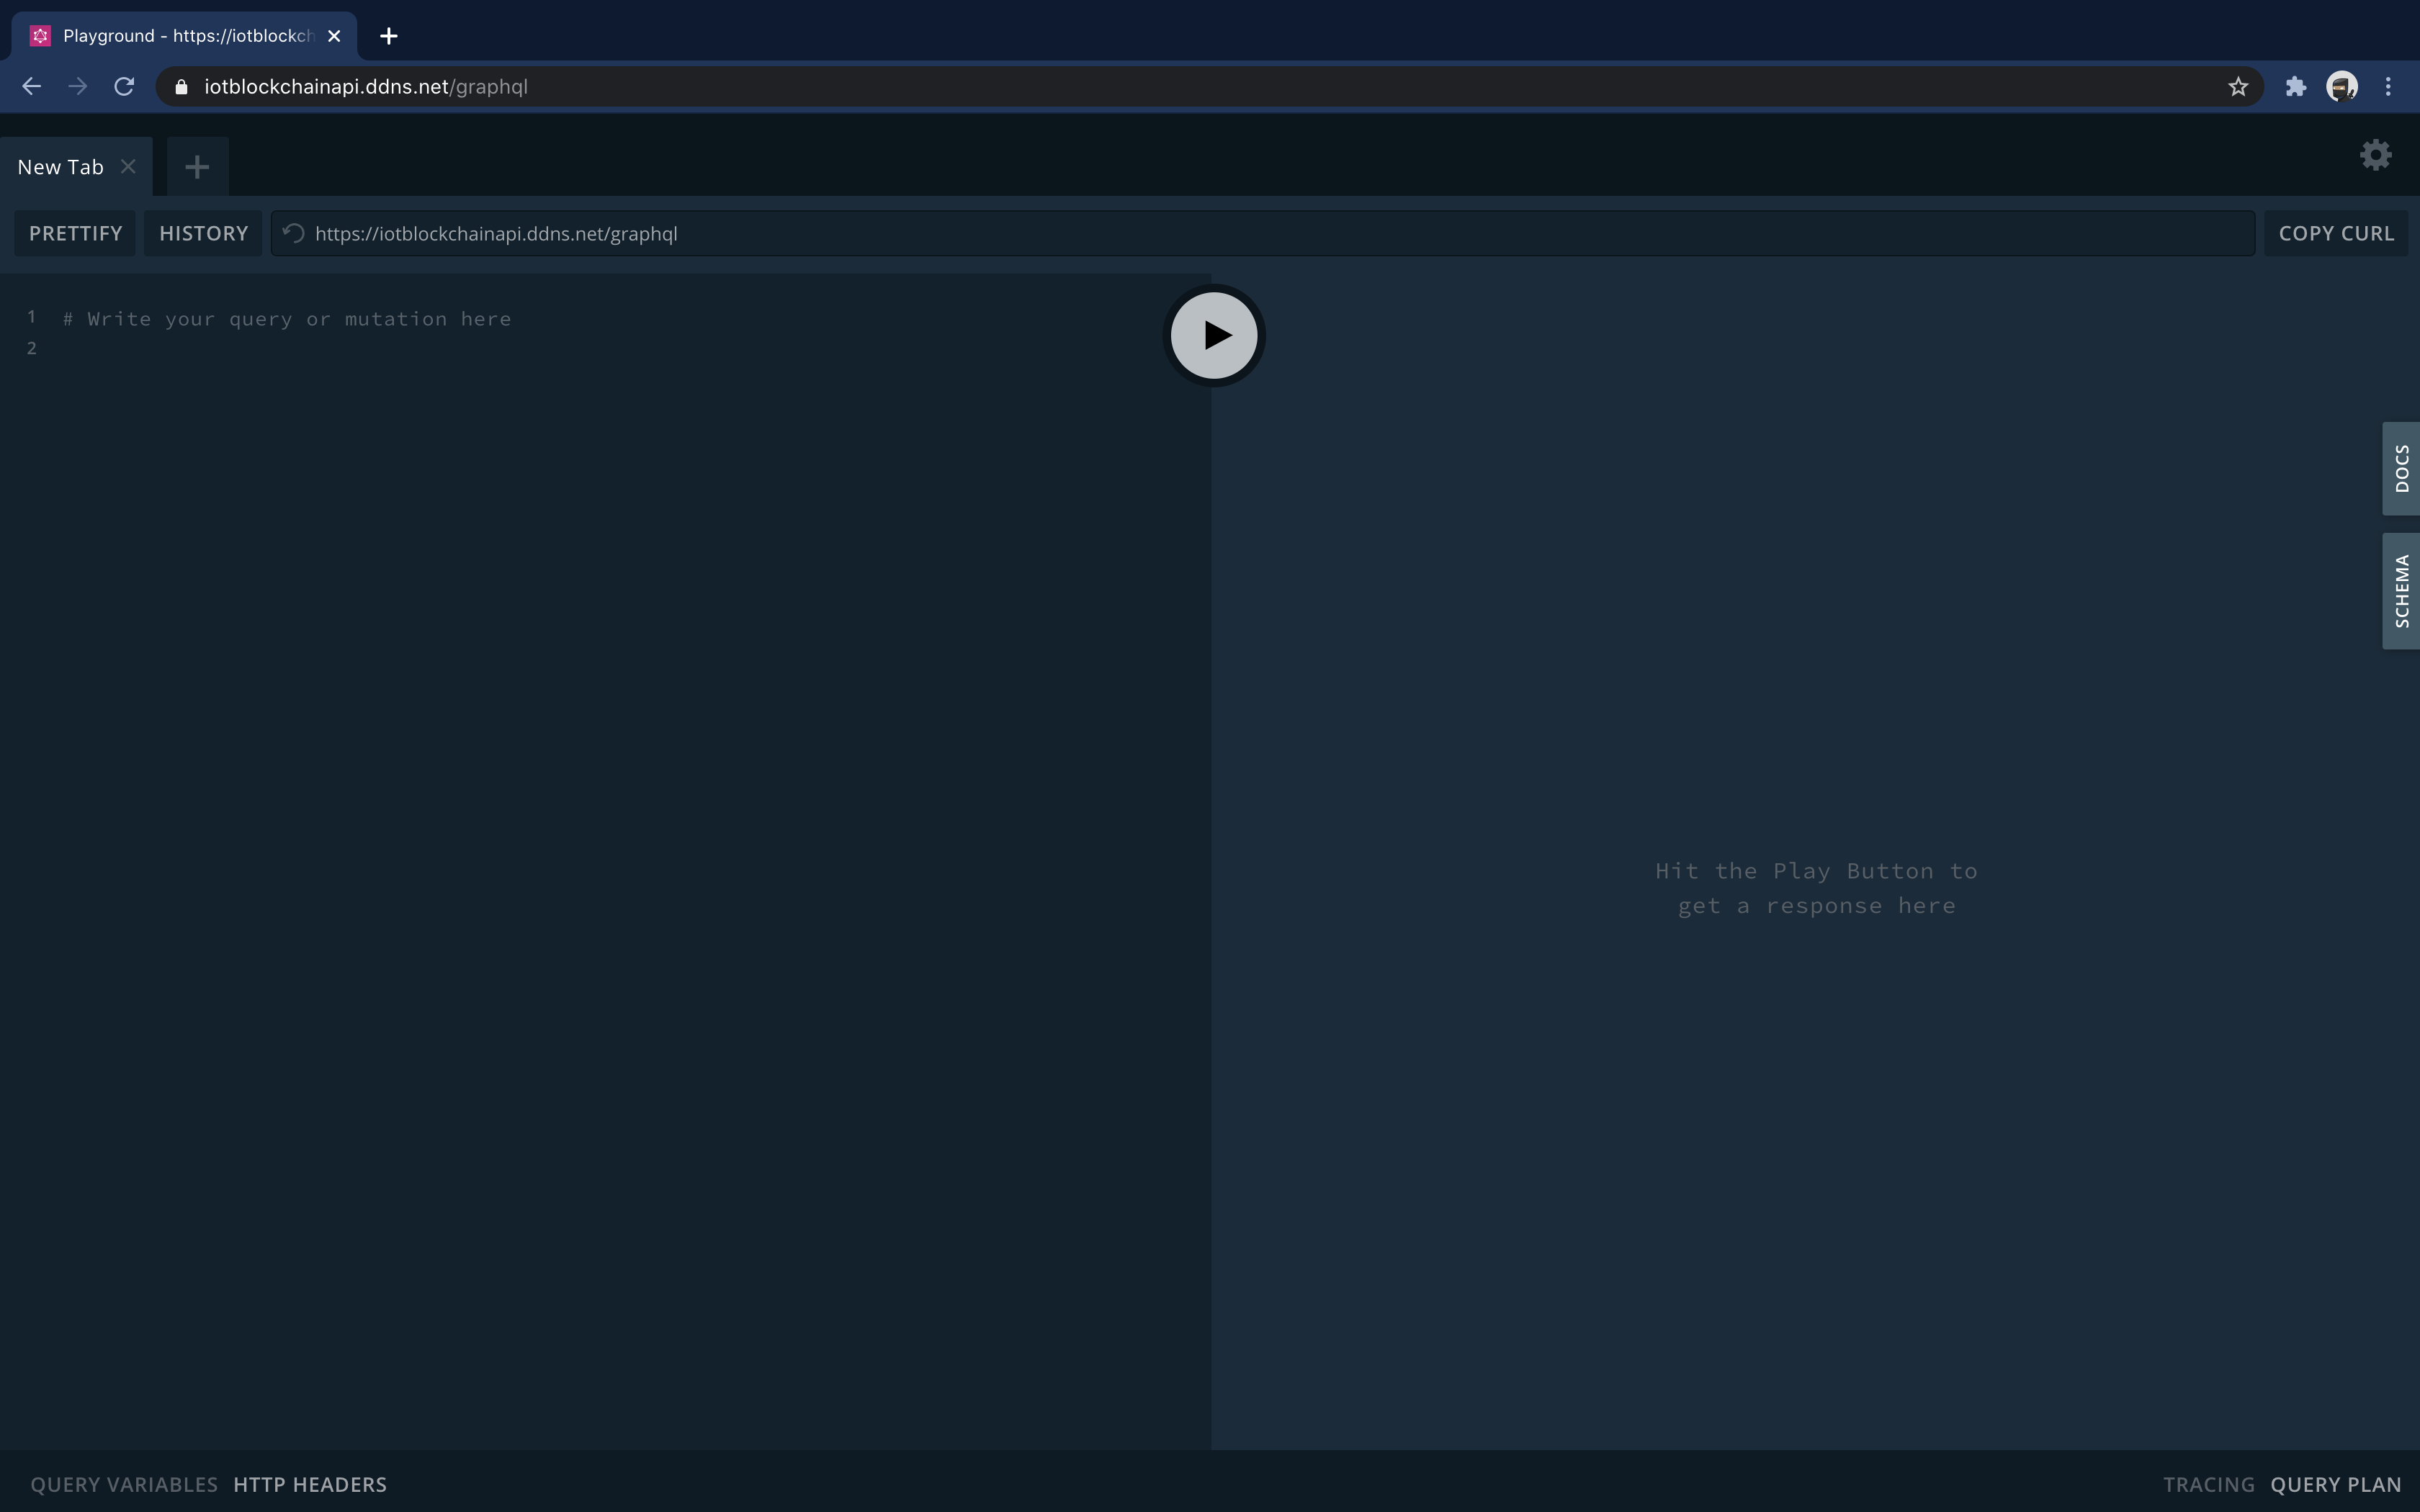
\includegraphics[width=\textwidth]{imagenes/desarrollo/web/api/graphql_api}
  \caption{GraphQL API endpoint.}
  \label{fig:graphql-api}
\end{figure}

\begin{figure}[h!]
  \centering
  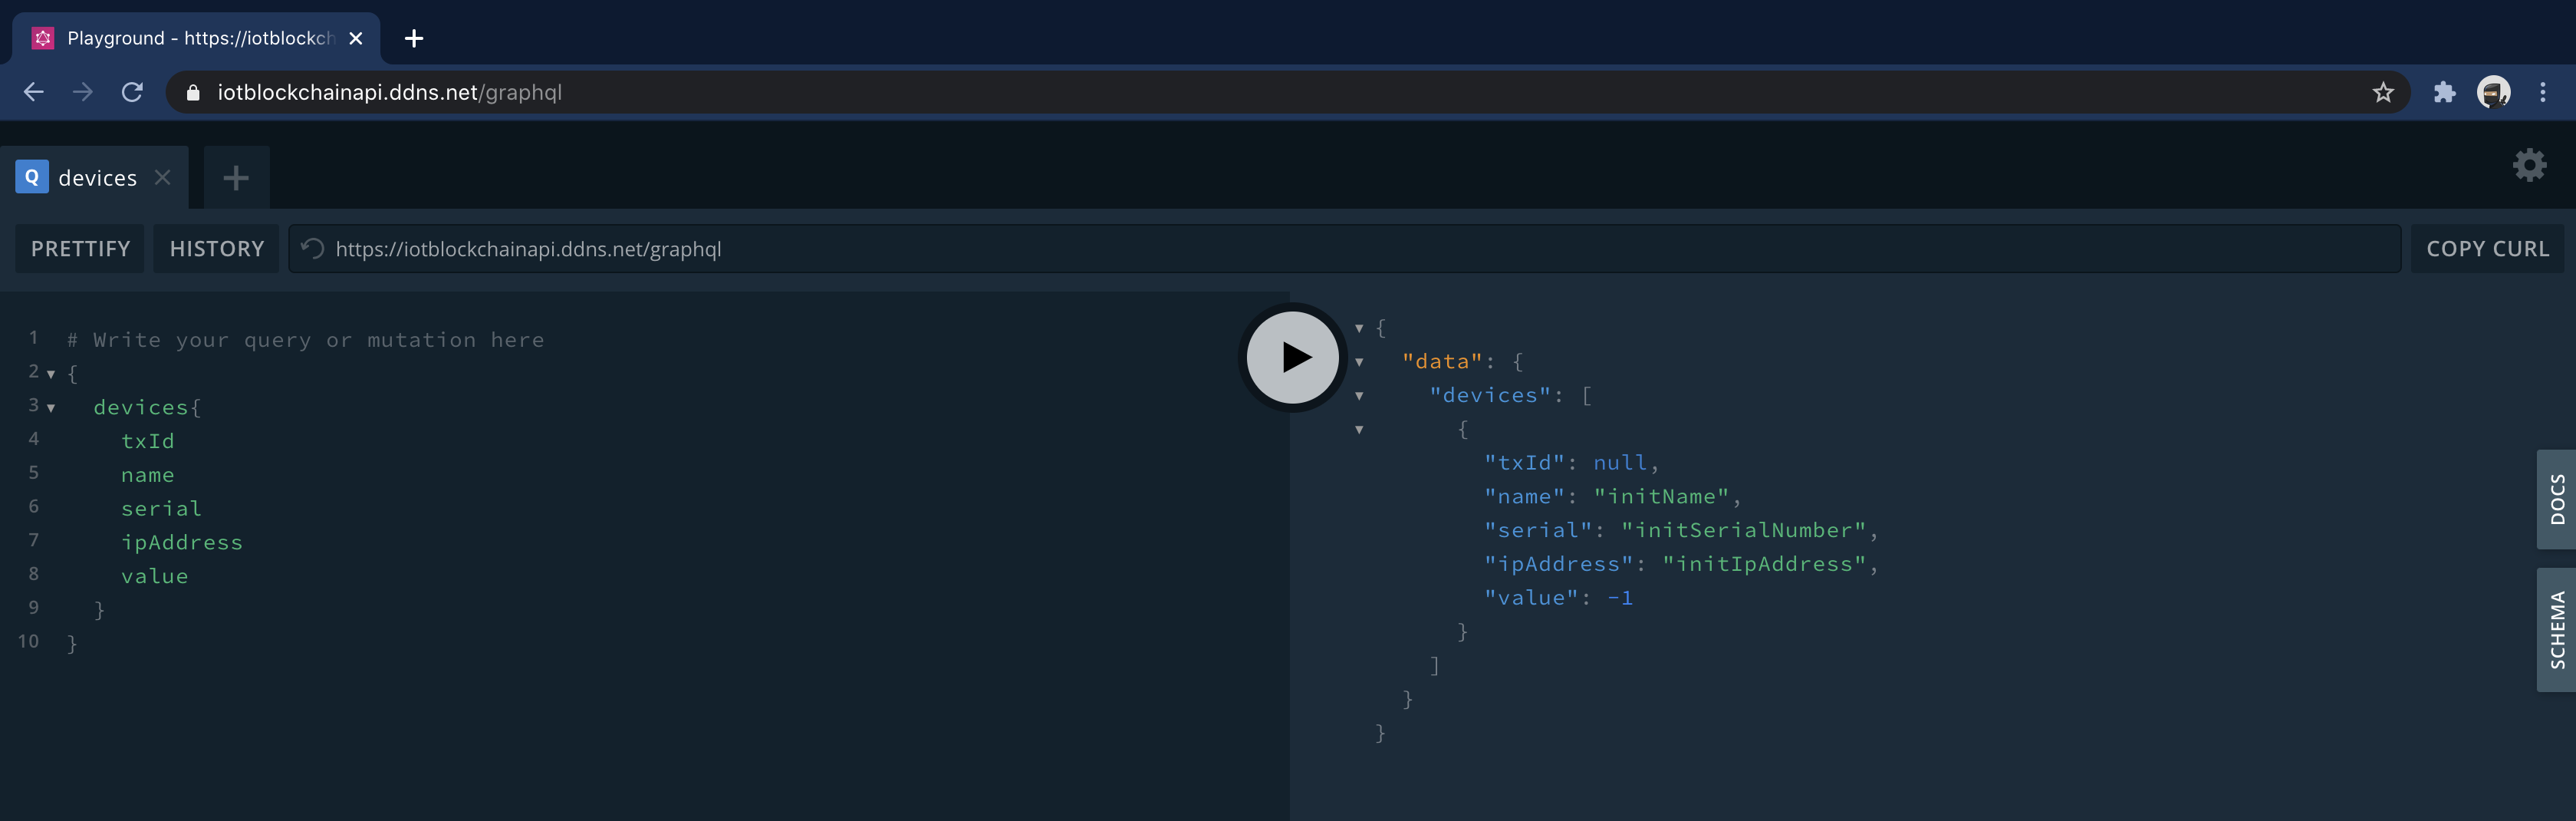
\includegraphics[width=\textwidth]{imagenes/desarrollo/web/api/graphql_query}
  \caption{Consulta a GraphQL API endpoint.}
  \label{fig:query-graphql-api}
\end{figure}

\begin{figure}[hbtp!]
  \begin{subfigure}{0.5\textwidth}
    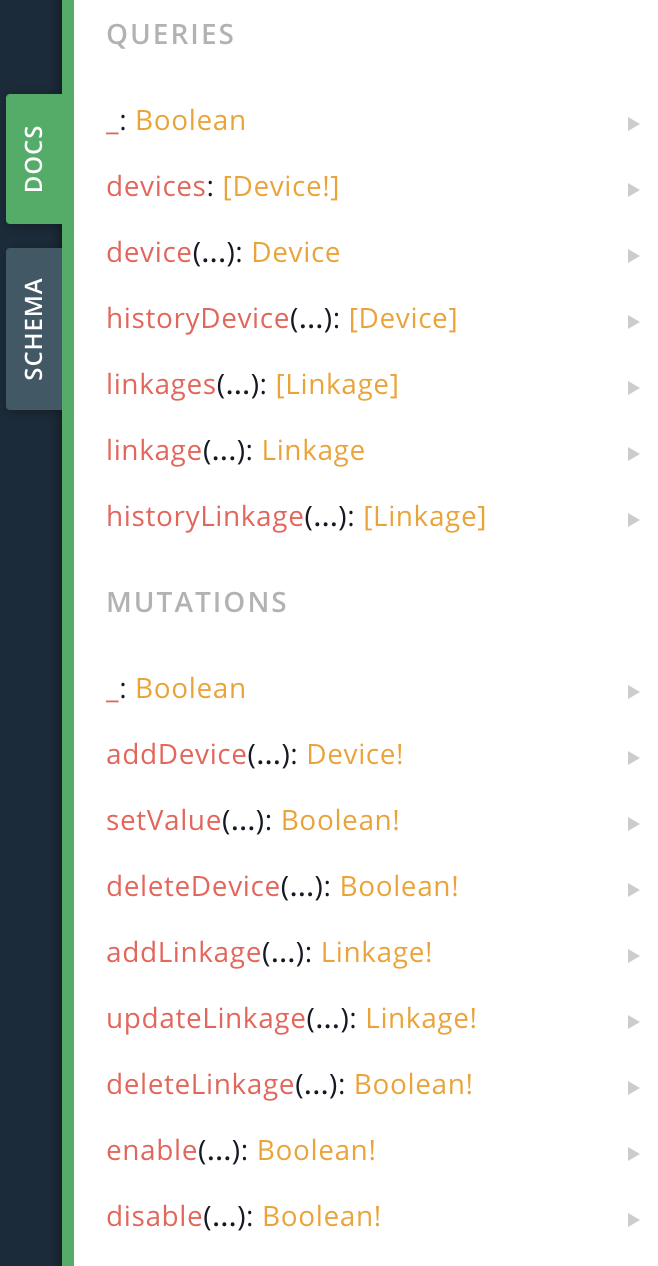
\includegraphics[width=\linewidth]{imagenes/desarrollo/web/api/graphql_docs}
    \caption{Docs GraphQL API.}
    \label{fig:graphql-docs}
  \end{subfigure}
  \begin{subfigure}{0.5\textwidth}
    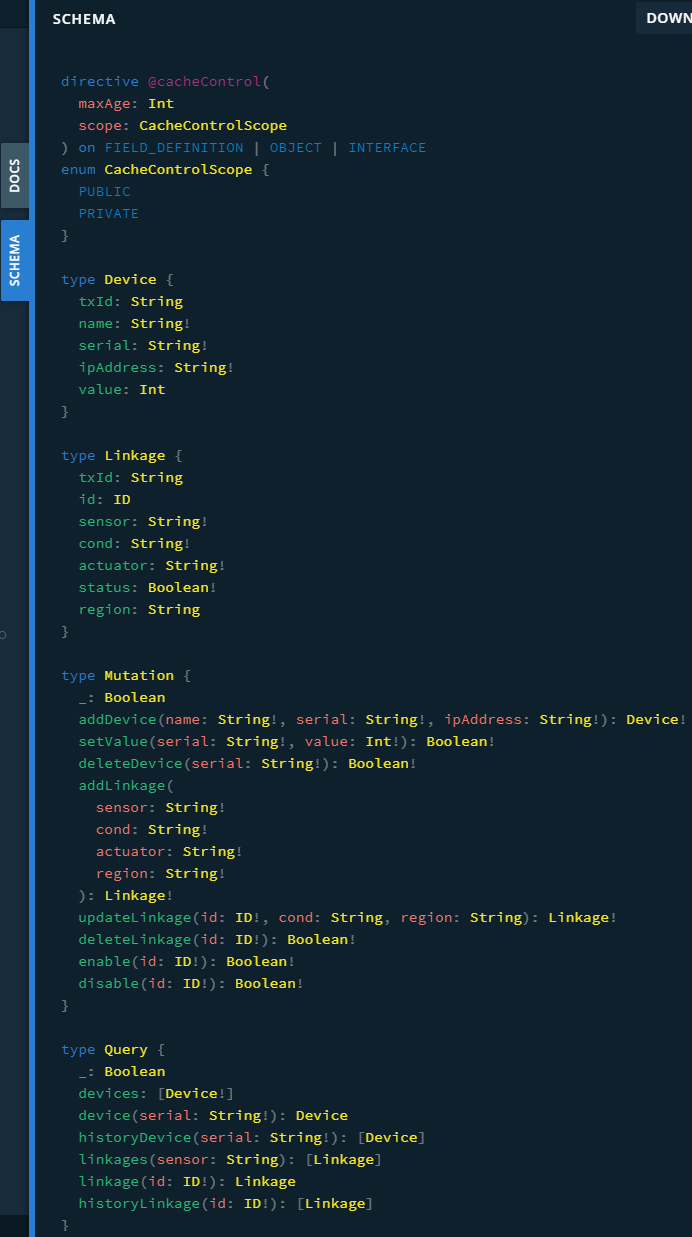
\includegraphics[width=\linewidth]{imagenes/desarrollo/web/api/graphql_schema}
    \caption{Schema GraphQL API.}
    \label{fig:graphql-schema}
  \end{subfigure}
  \caption{Información de GraphQL API.}
  \label{fig:info-graphql}
\end{figure}

\newpage

\subsection{Vista del Front end.}

\begin{figure}[h!]
  \centering
  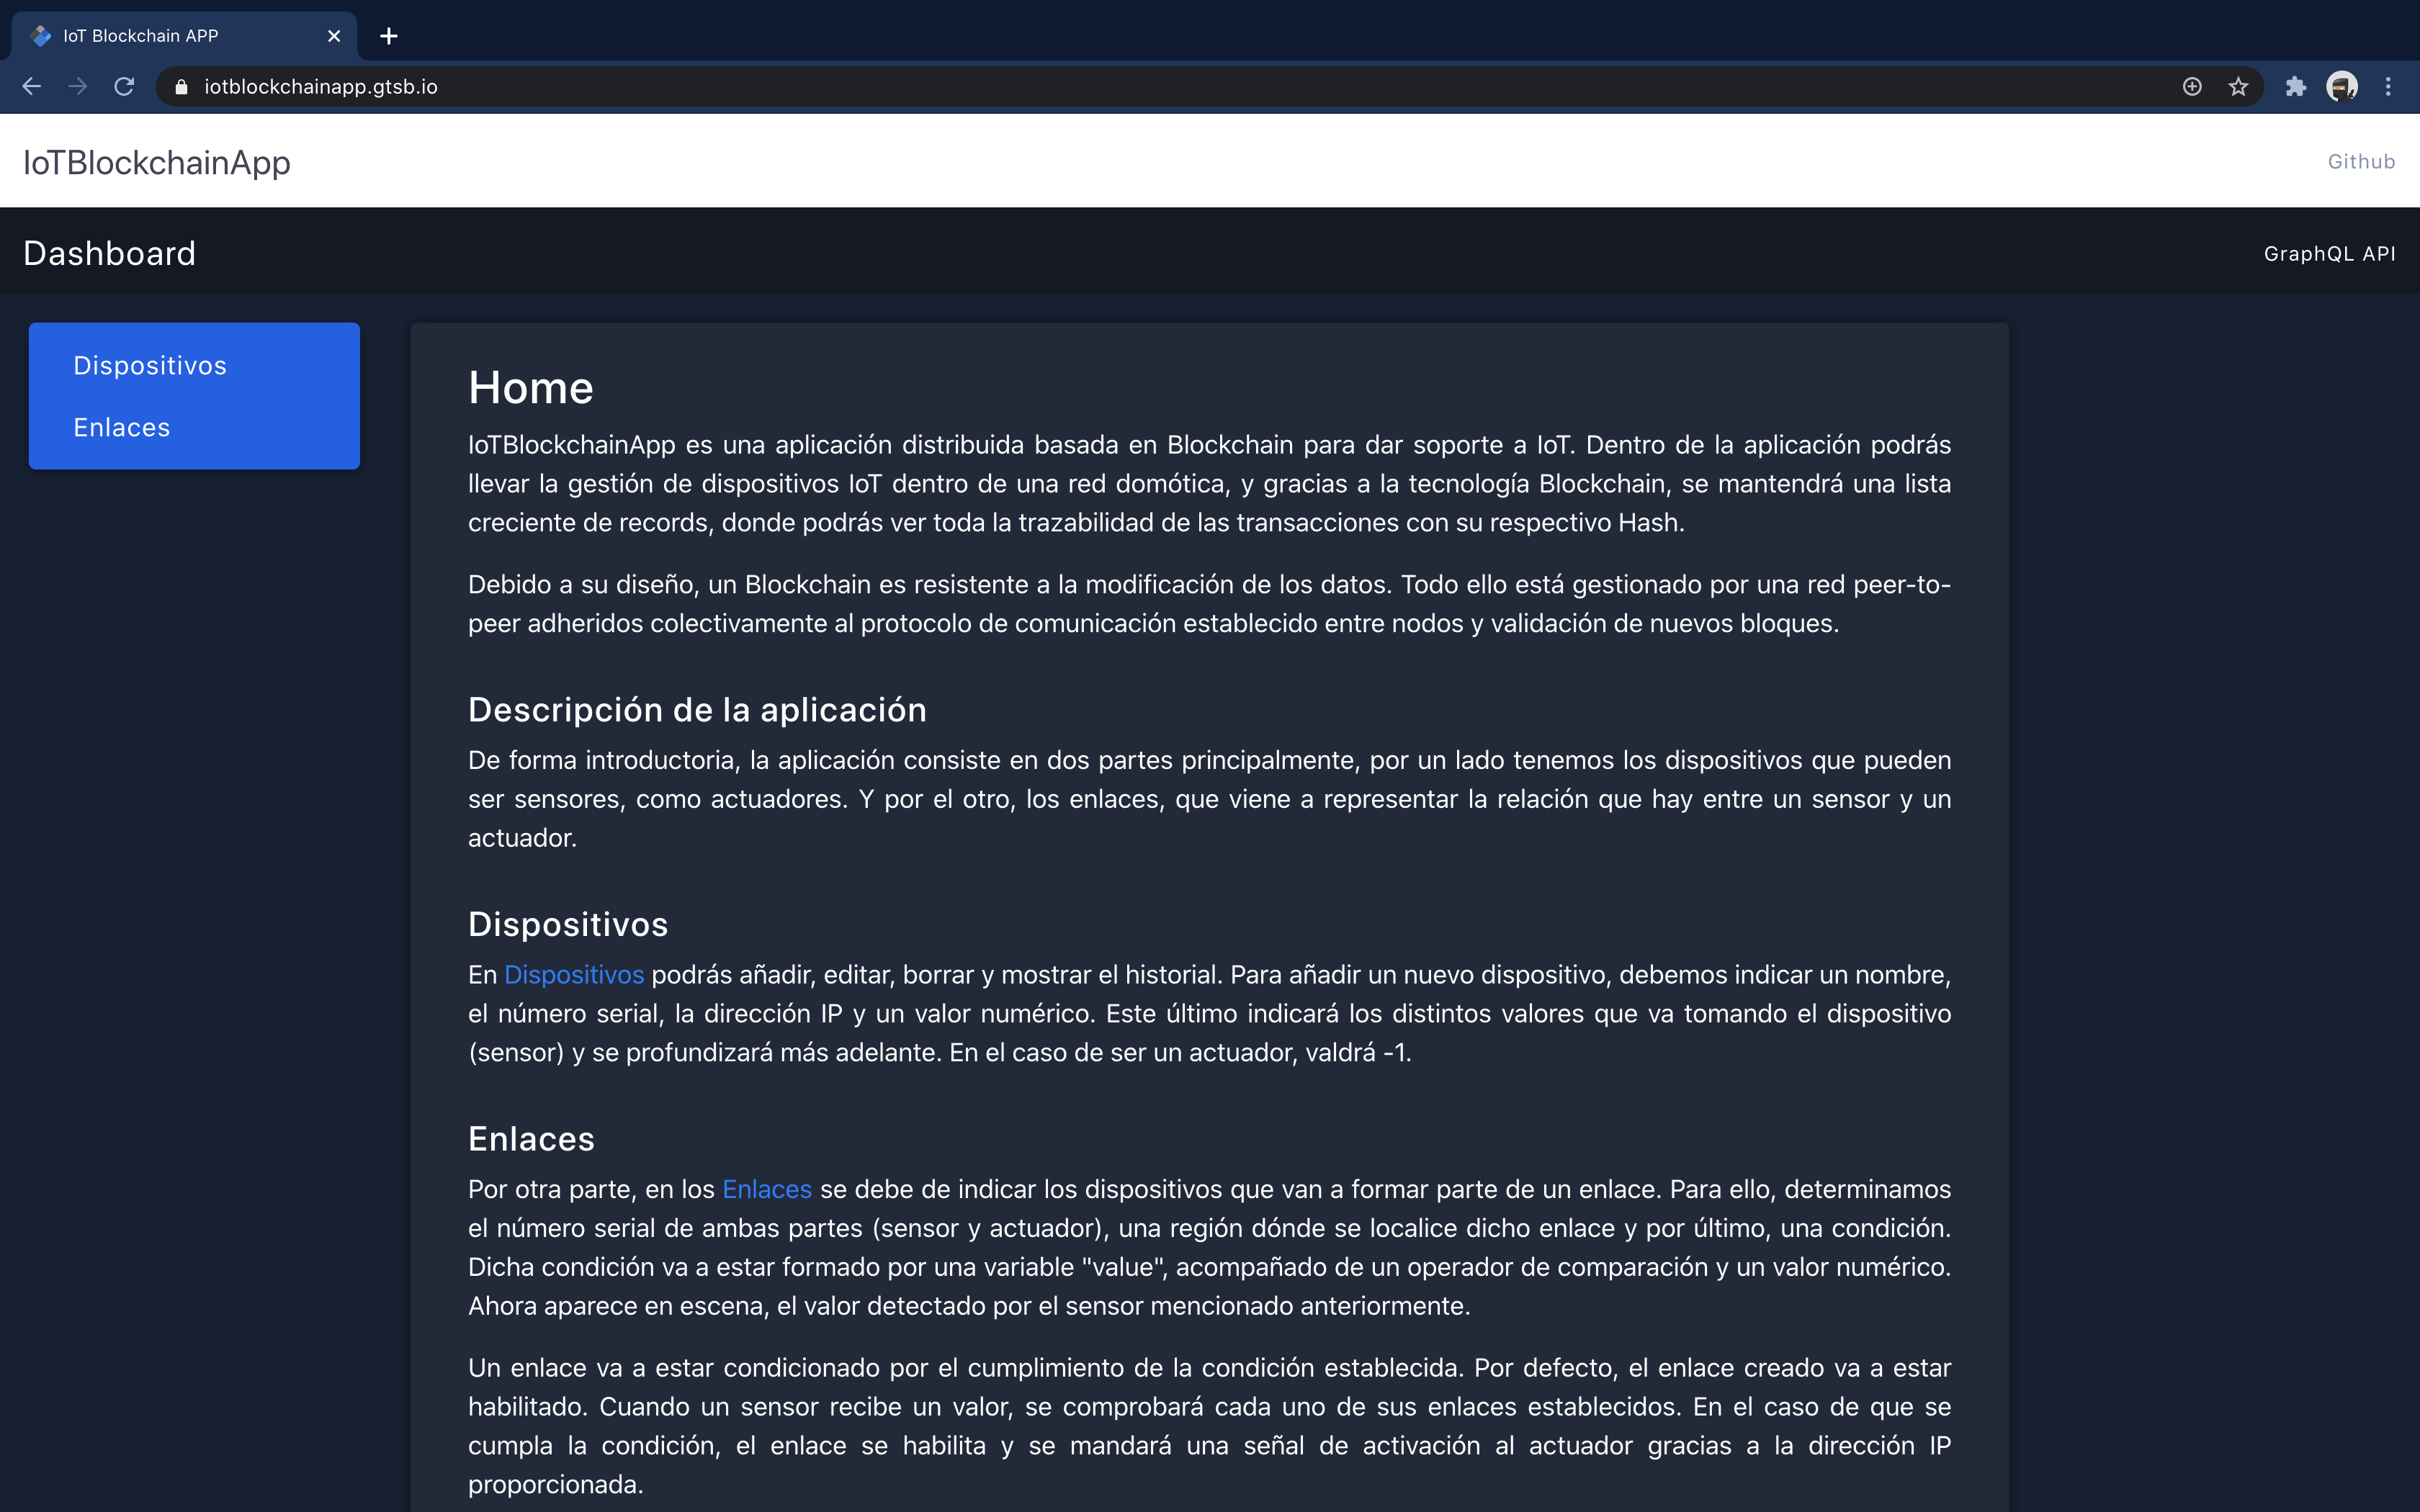
\includegraphics[width=\textwidth]{imagenes/desarrollo/web/pagina_inicial}
  \caption{Página inicial.}
  \label{fig:pagina-inicial}
\end{figure}

\subsubsection*{Vista dispositivo.}

\begin{figure}[h!]
  \centering
  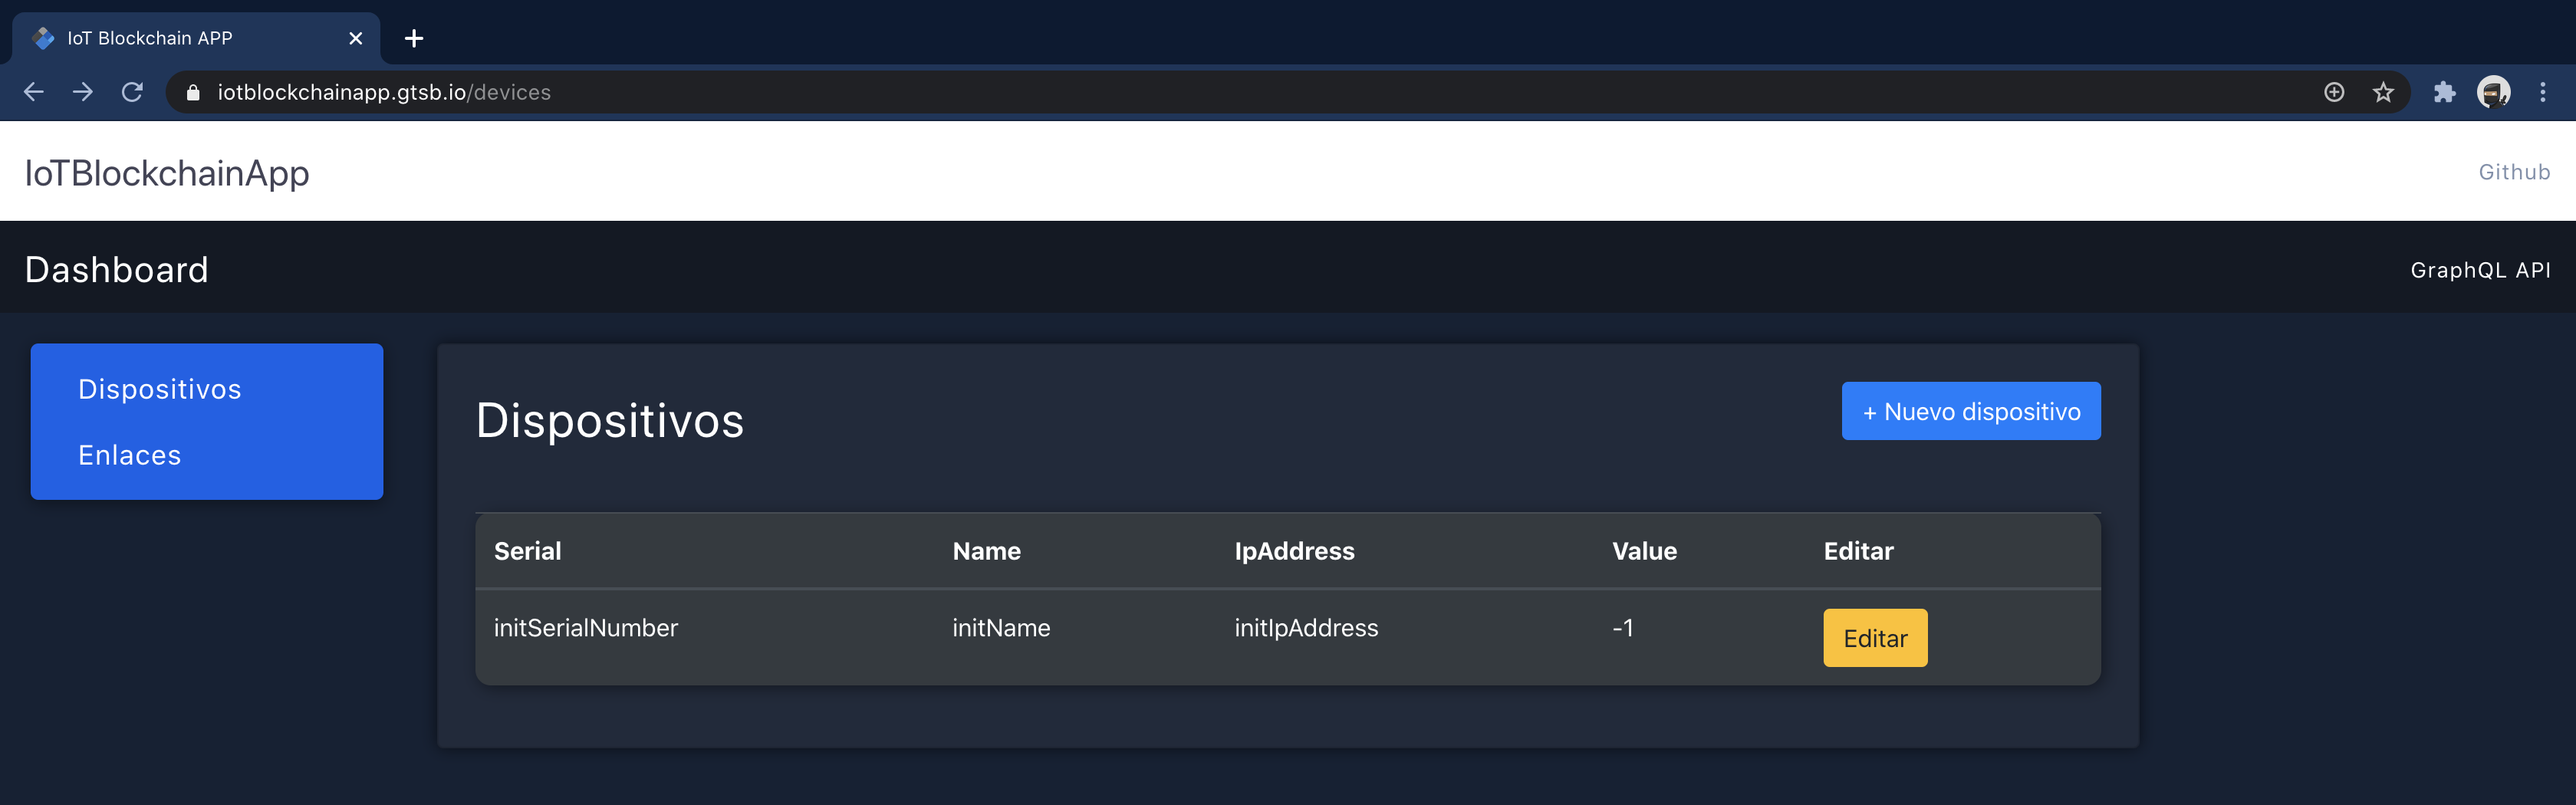
\includegraphics[width=\textwidth]{imagenes/desarrollo/web/vista_dispositivos}
  \caption{Vista dispositivos.}
  \label{fig:vista-dispositivo}
\end{figure}

\begin{figure}[h!]
 \centering
  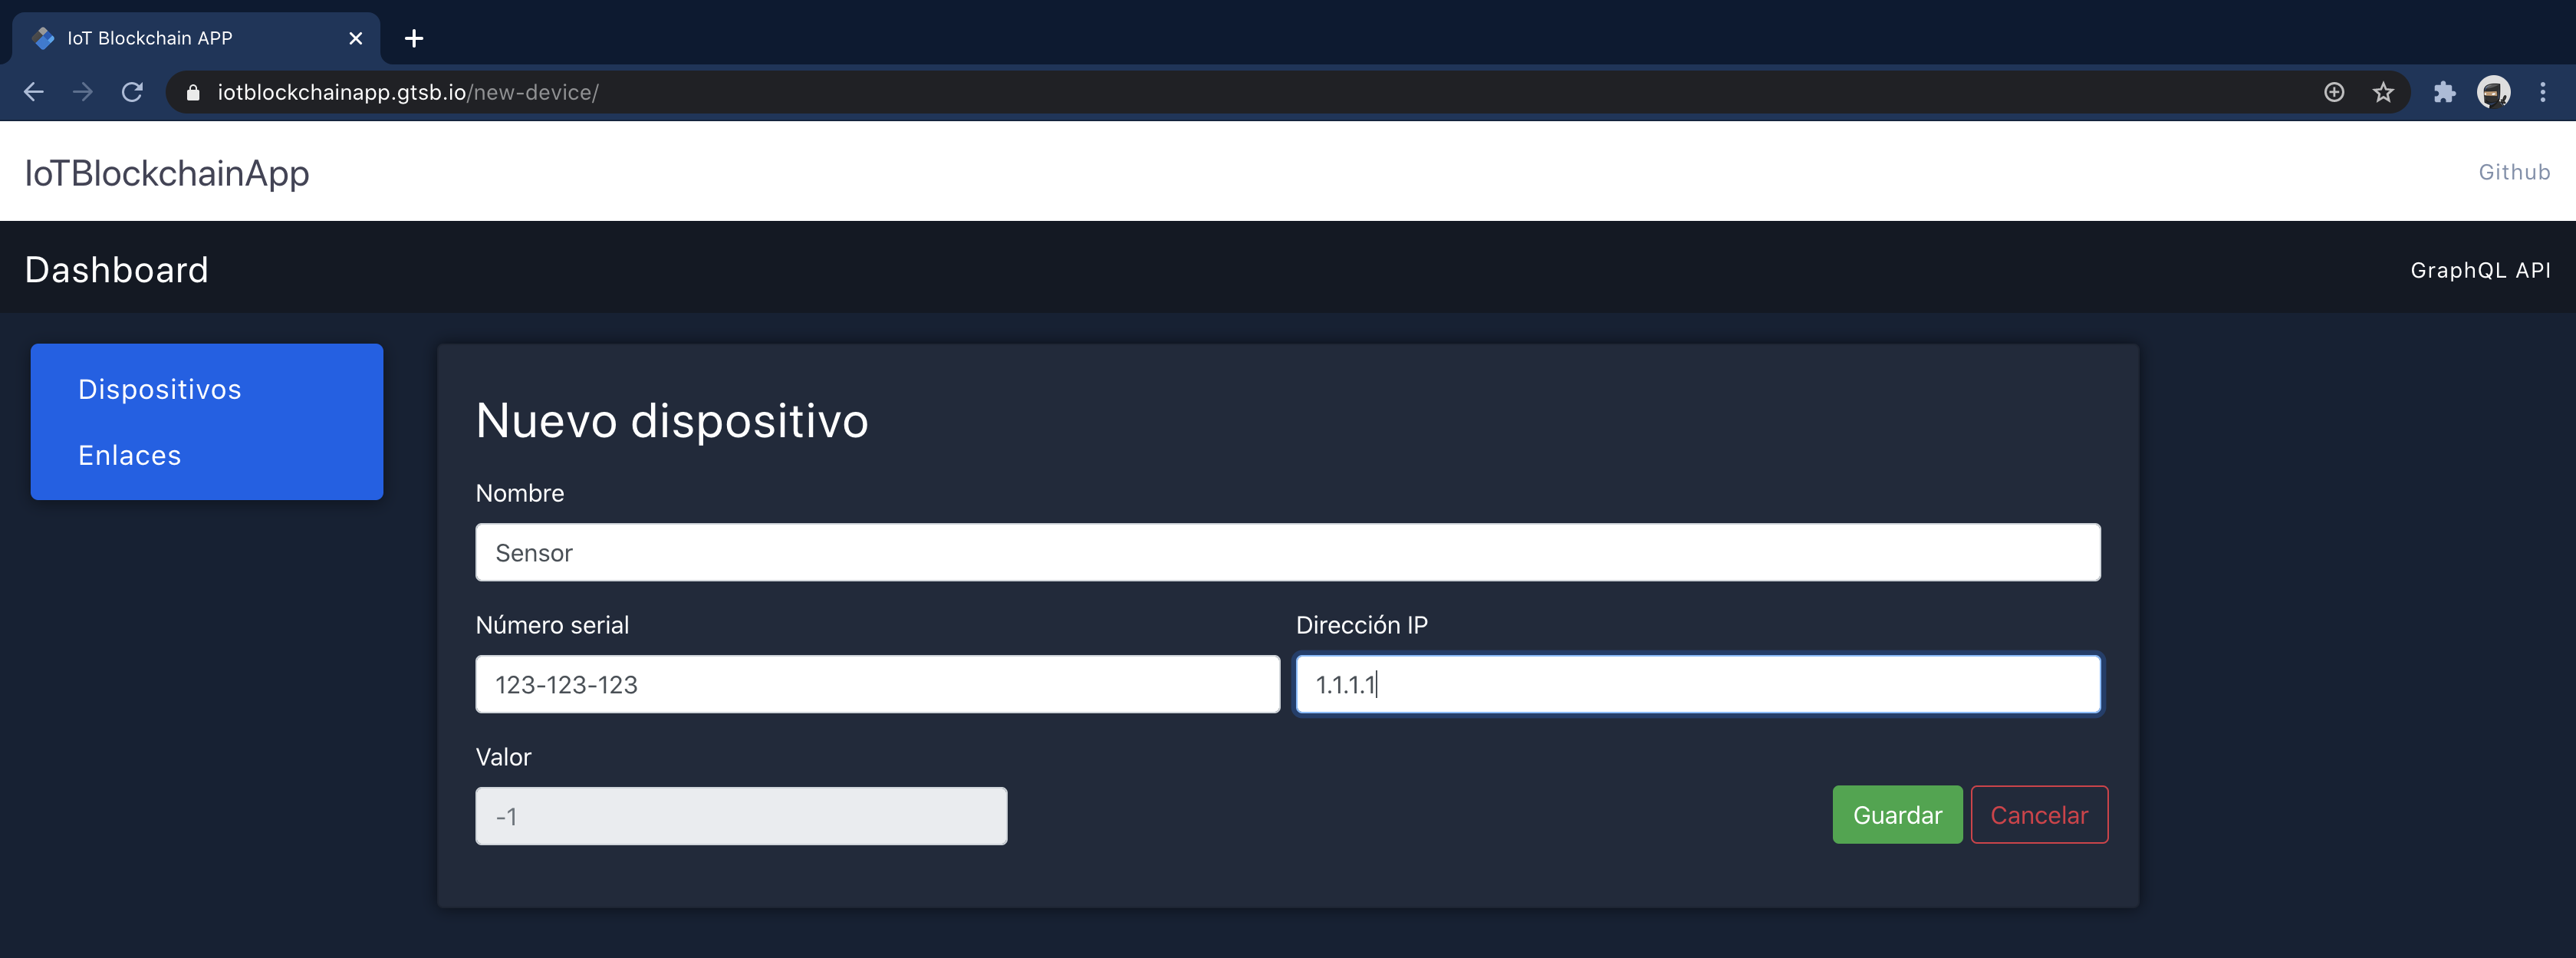
\includegraphics[width=\textwidth]{imagenes/desarrollo/web/aniadir_dispositivo}
  \caption{Añadir dispositivo.}
  \label{fig:aniadir-dispositivo}
\end{figure}

\begin{figure}[h!]
  \centering
  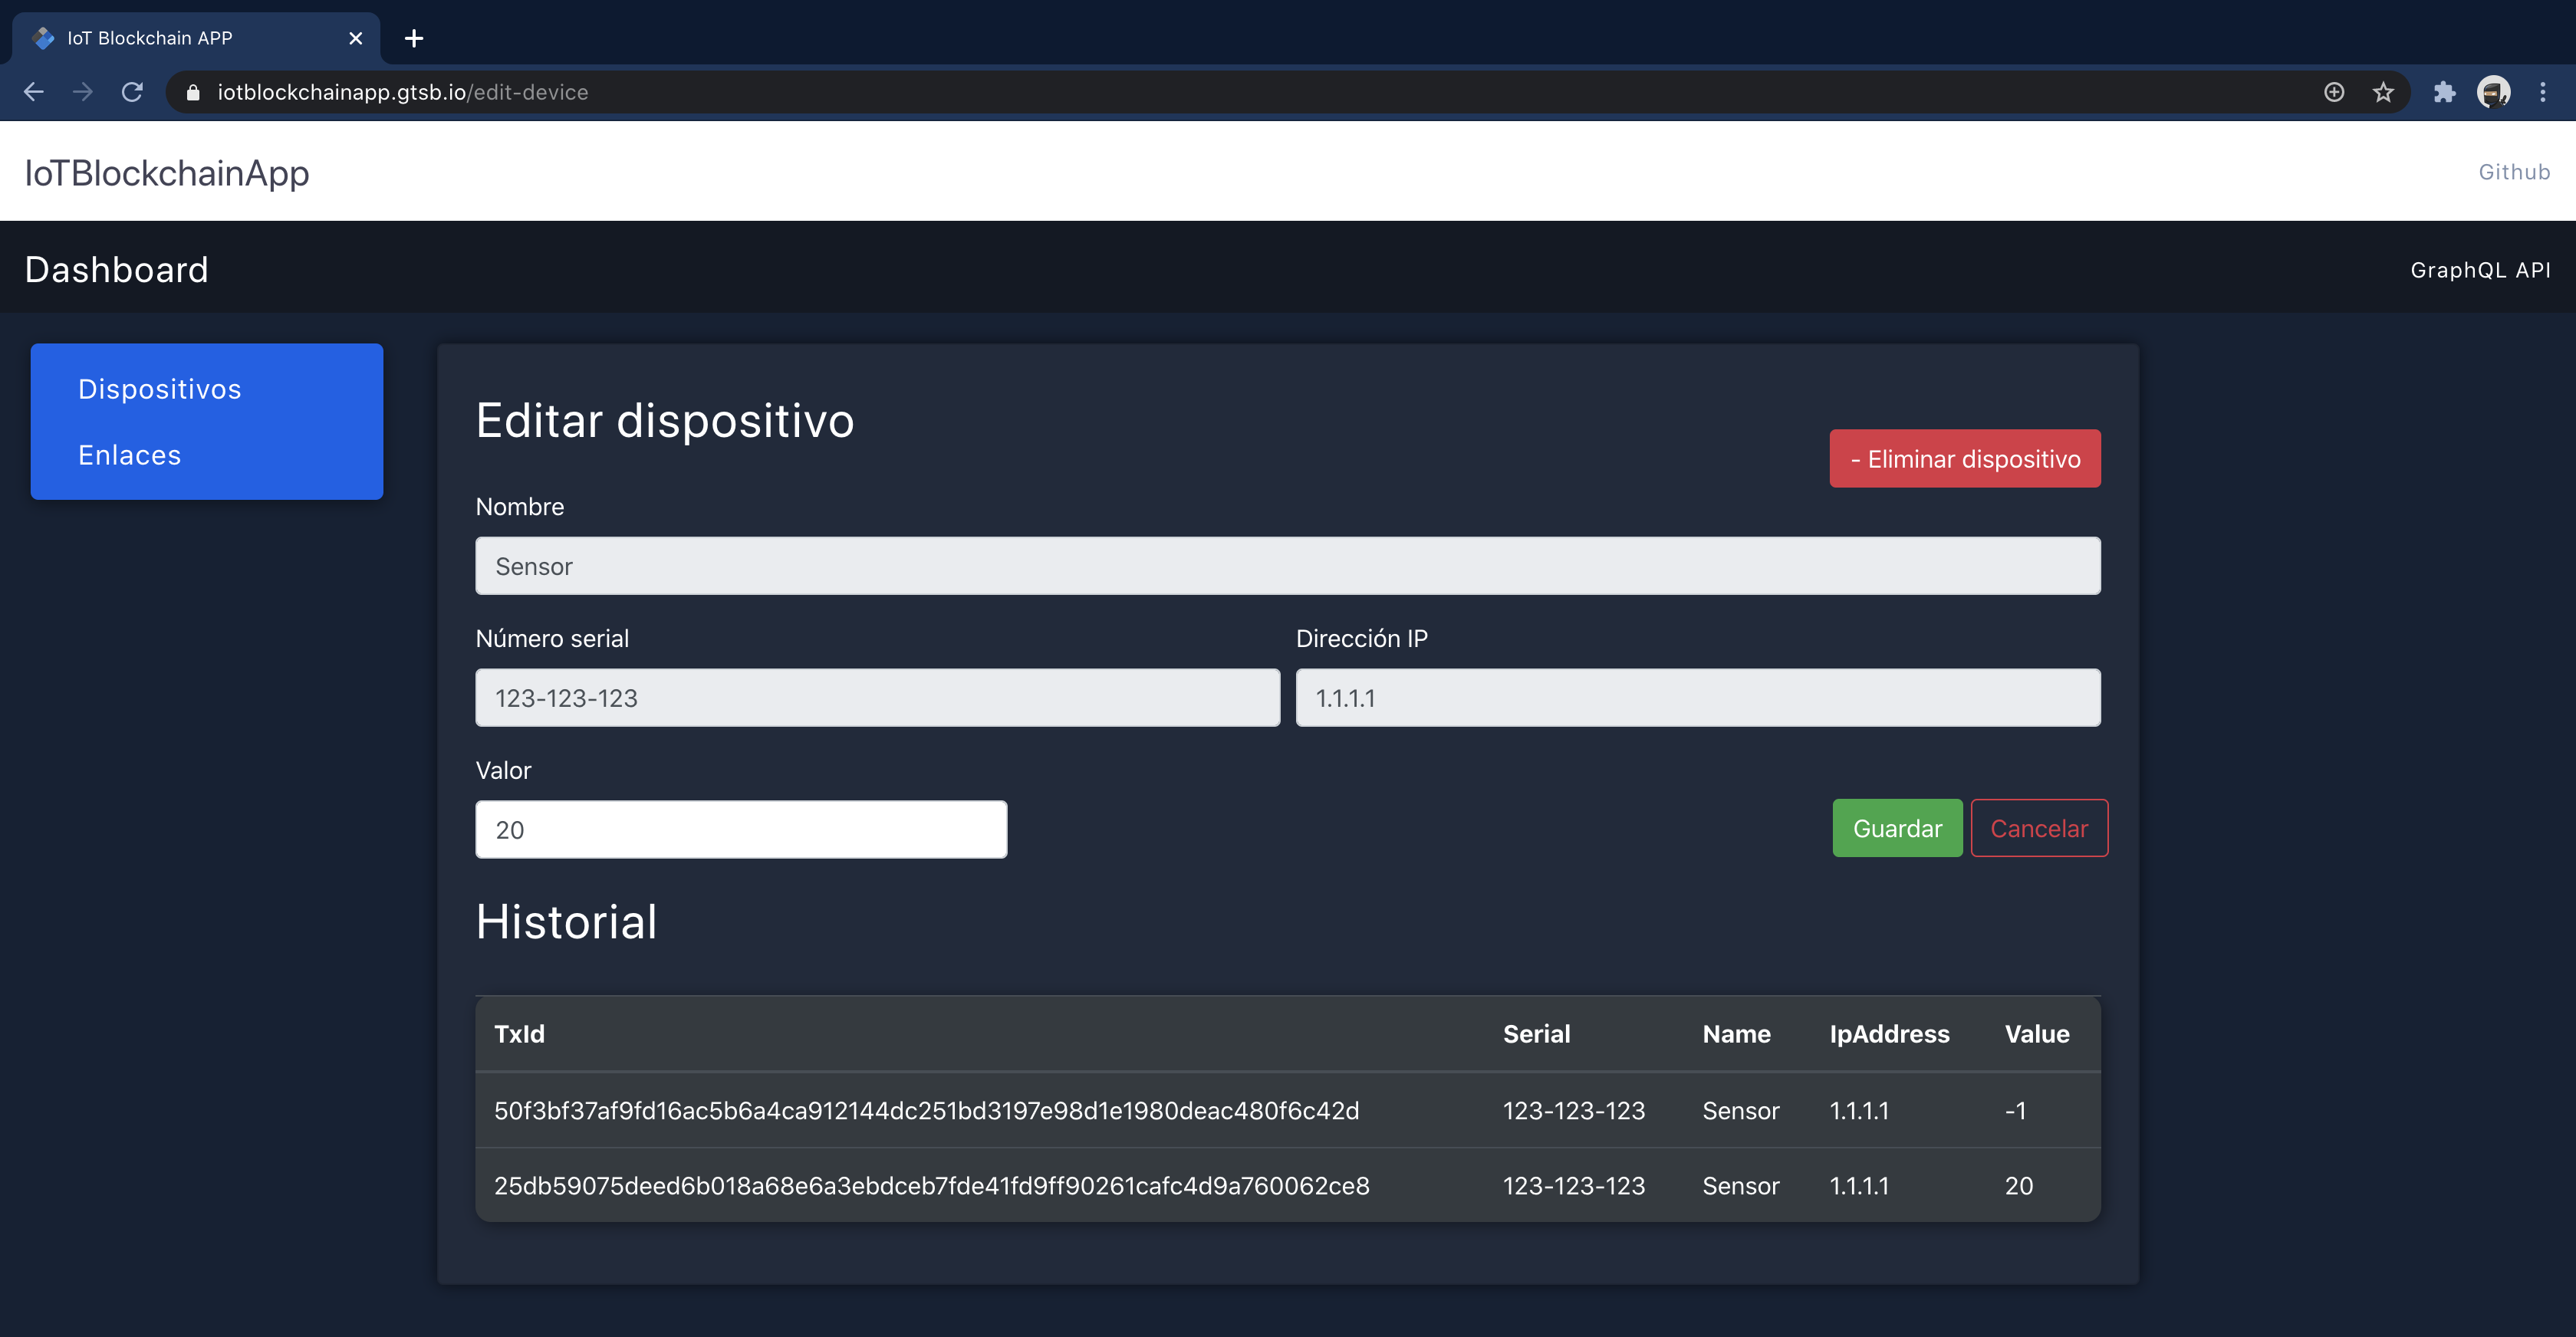
\includegraphics[width=\textwidth]{imagenes/desarrollo/web/editar_dispositivo}
  \caption{Editar dispositivo.}
  \label{fig:editar-dispositivo}
\end{figure}

\newpage

\subsubsection*{Vista enlace.}

\begin{figure}[h!]
  \centering
  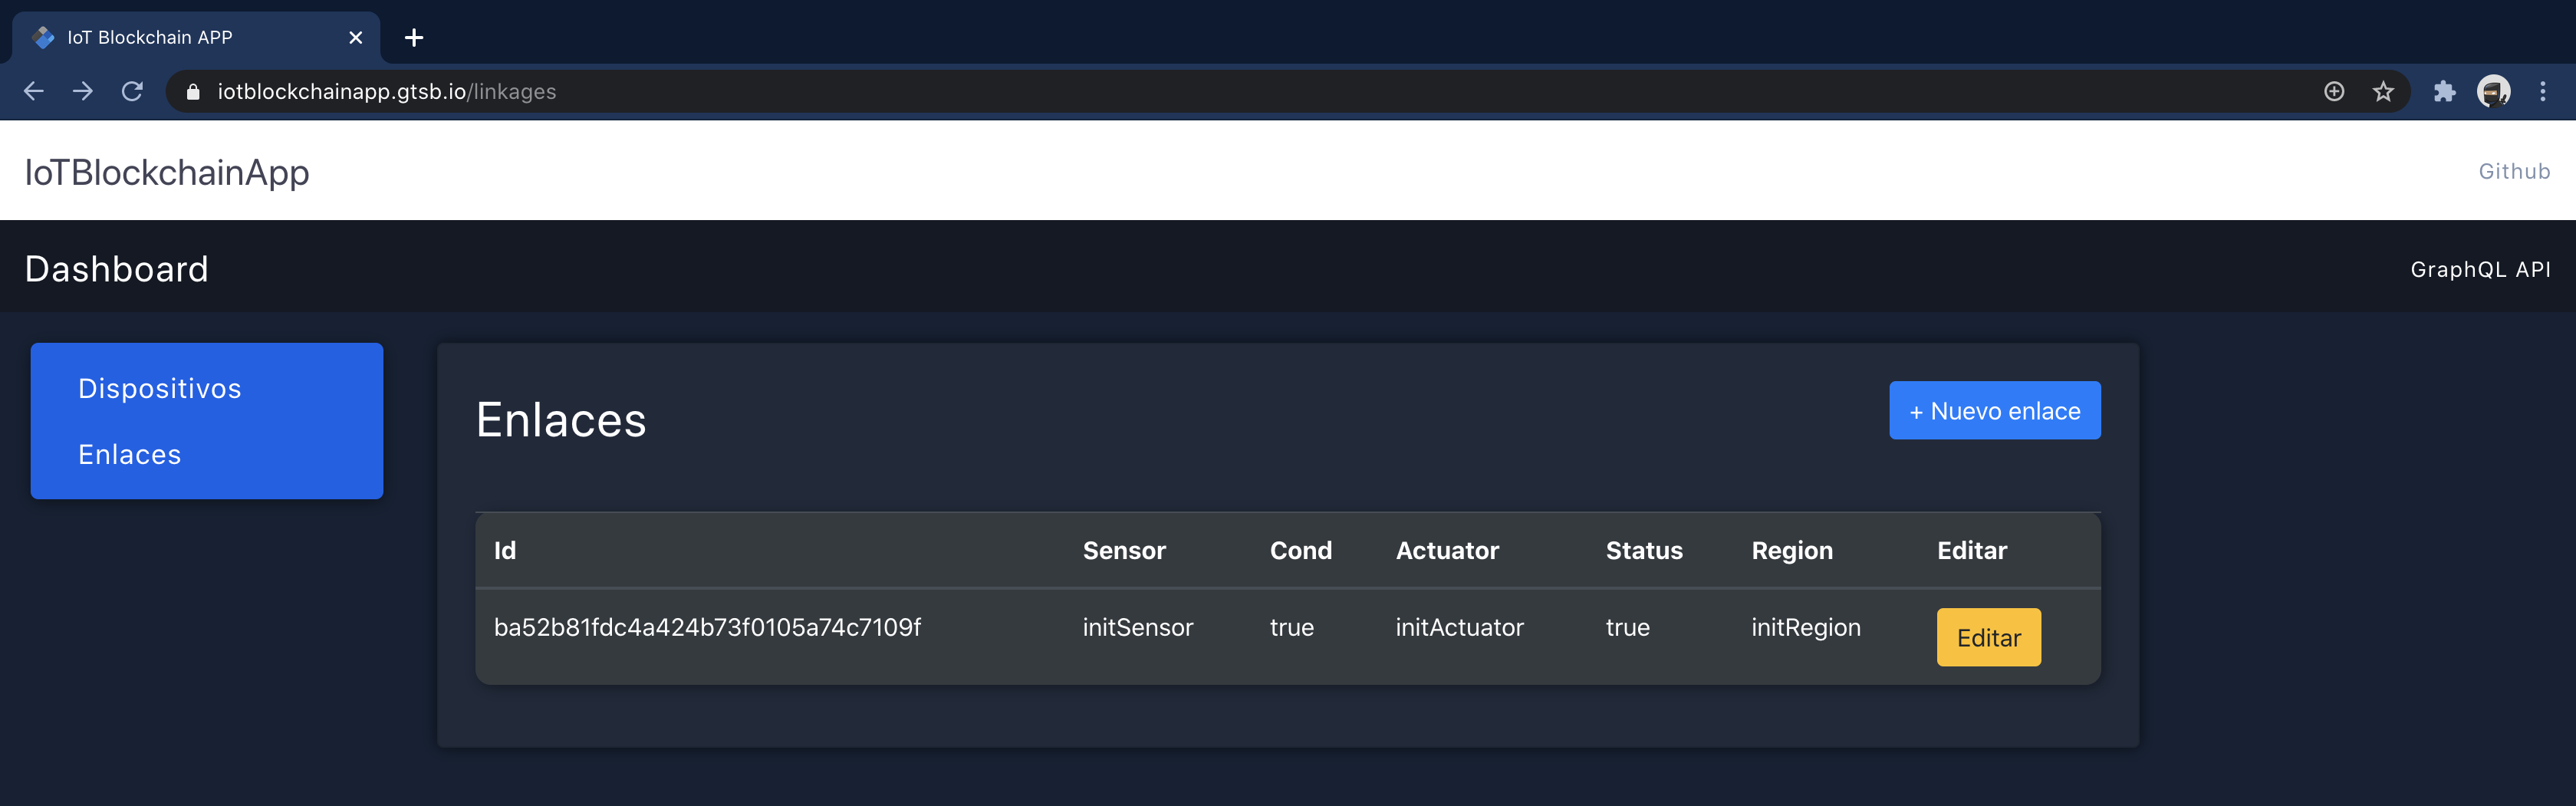
\includegraphics[width=\textwidth]{imagenes/desarrollo/web/vista_enlaces}
  \caption{Vista enlaces.}
  \label{fig:vista-enlace}
\end{figure}

\begin{figure}[h!]
  \centering
  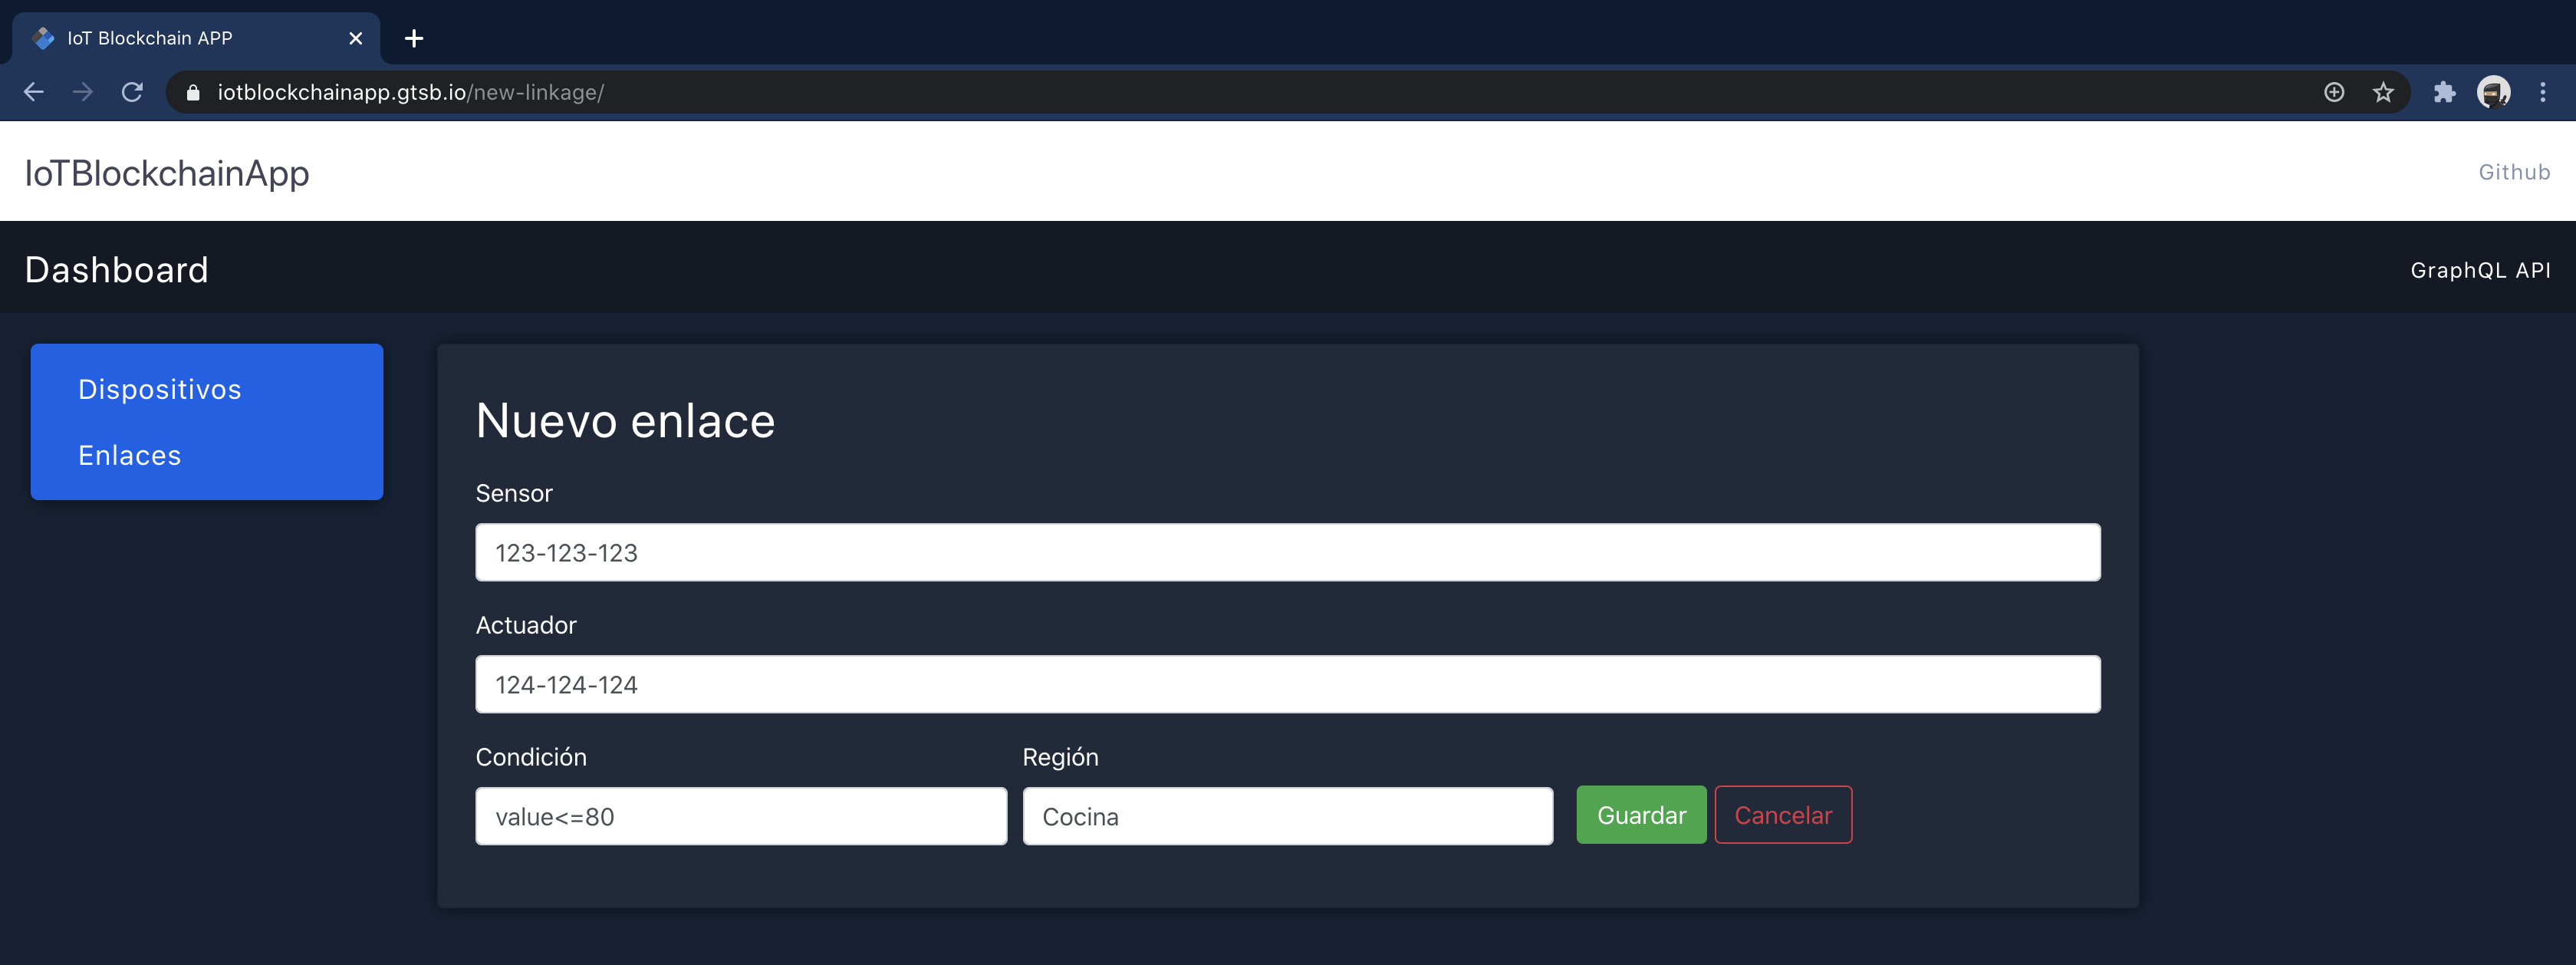
\includegraphics[width=\textwidth]{imagenes/desarrollo/web/aniadir_enlace}
  \caption{Añadir enlace.}
  \label{fig:aniadir-enlace}
\end{figure}

\begin{figure}[h!]
  \centering
  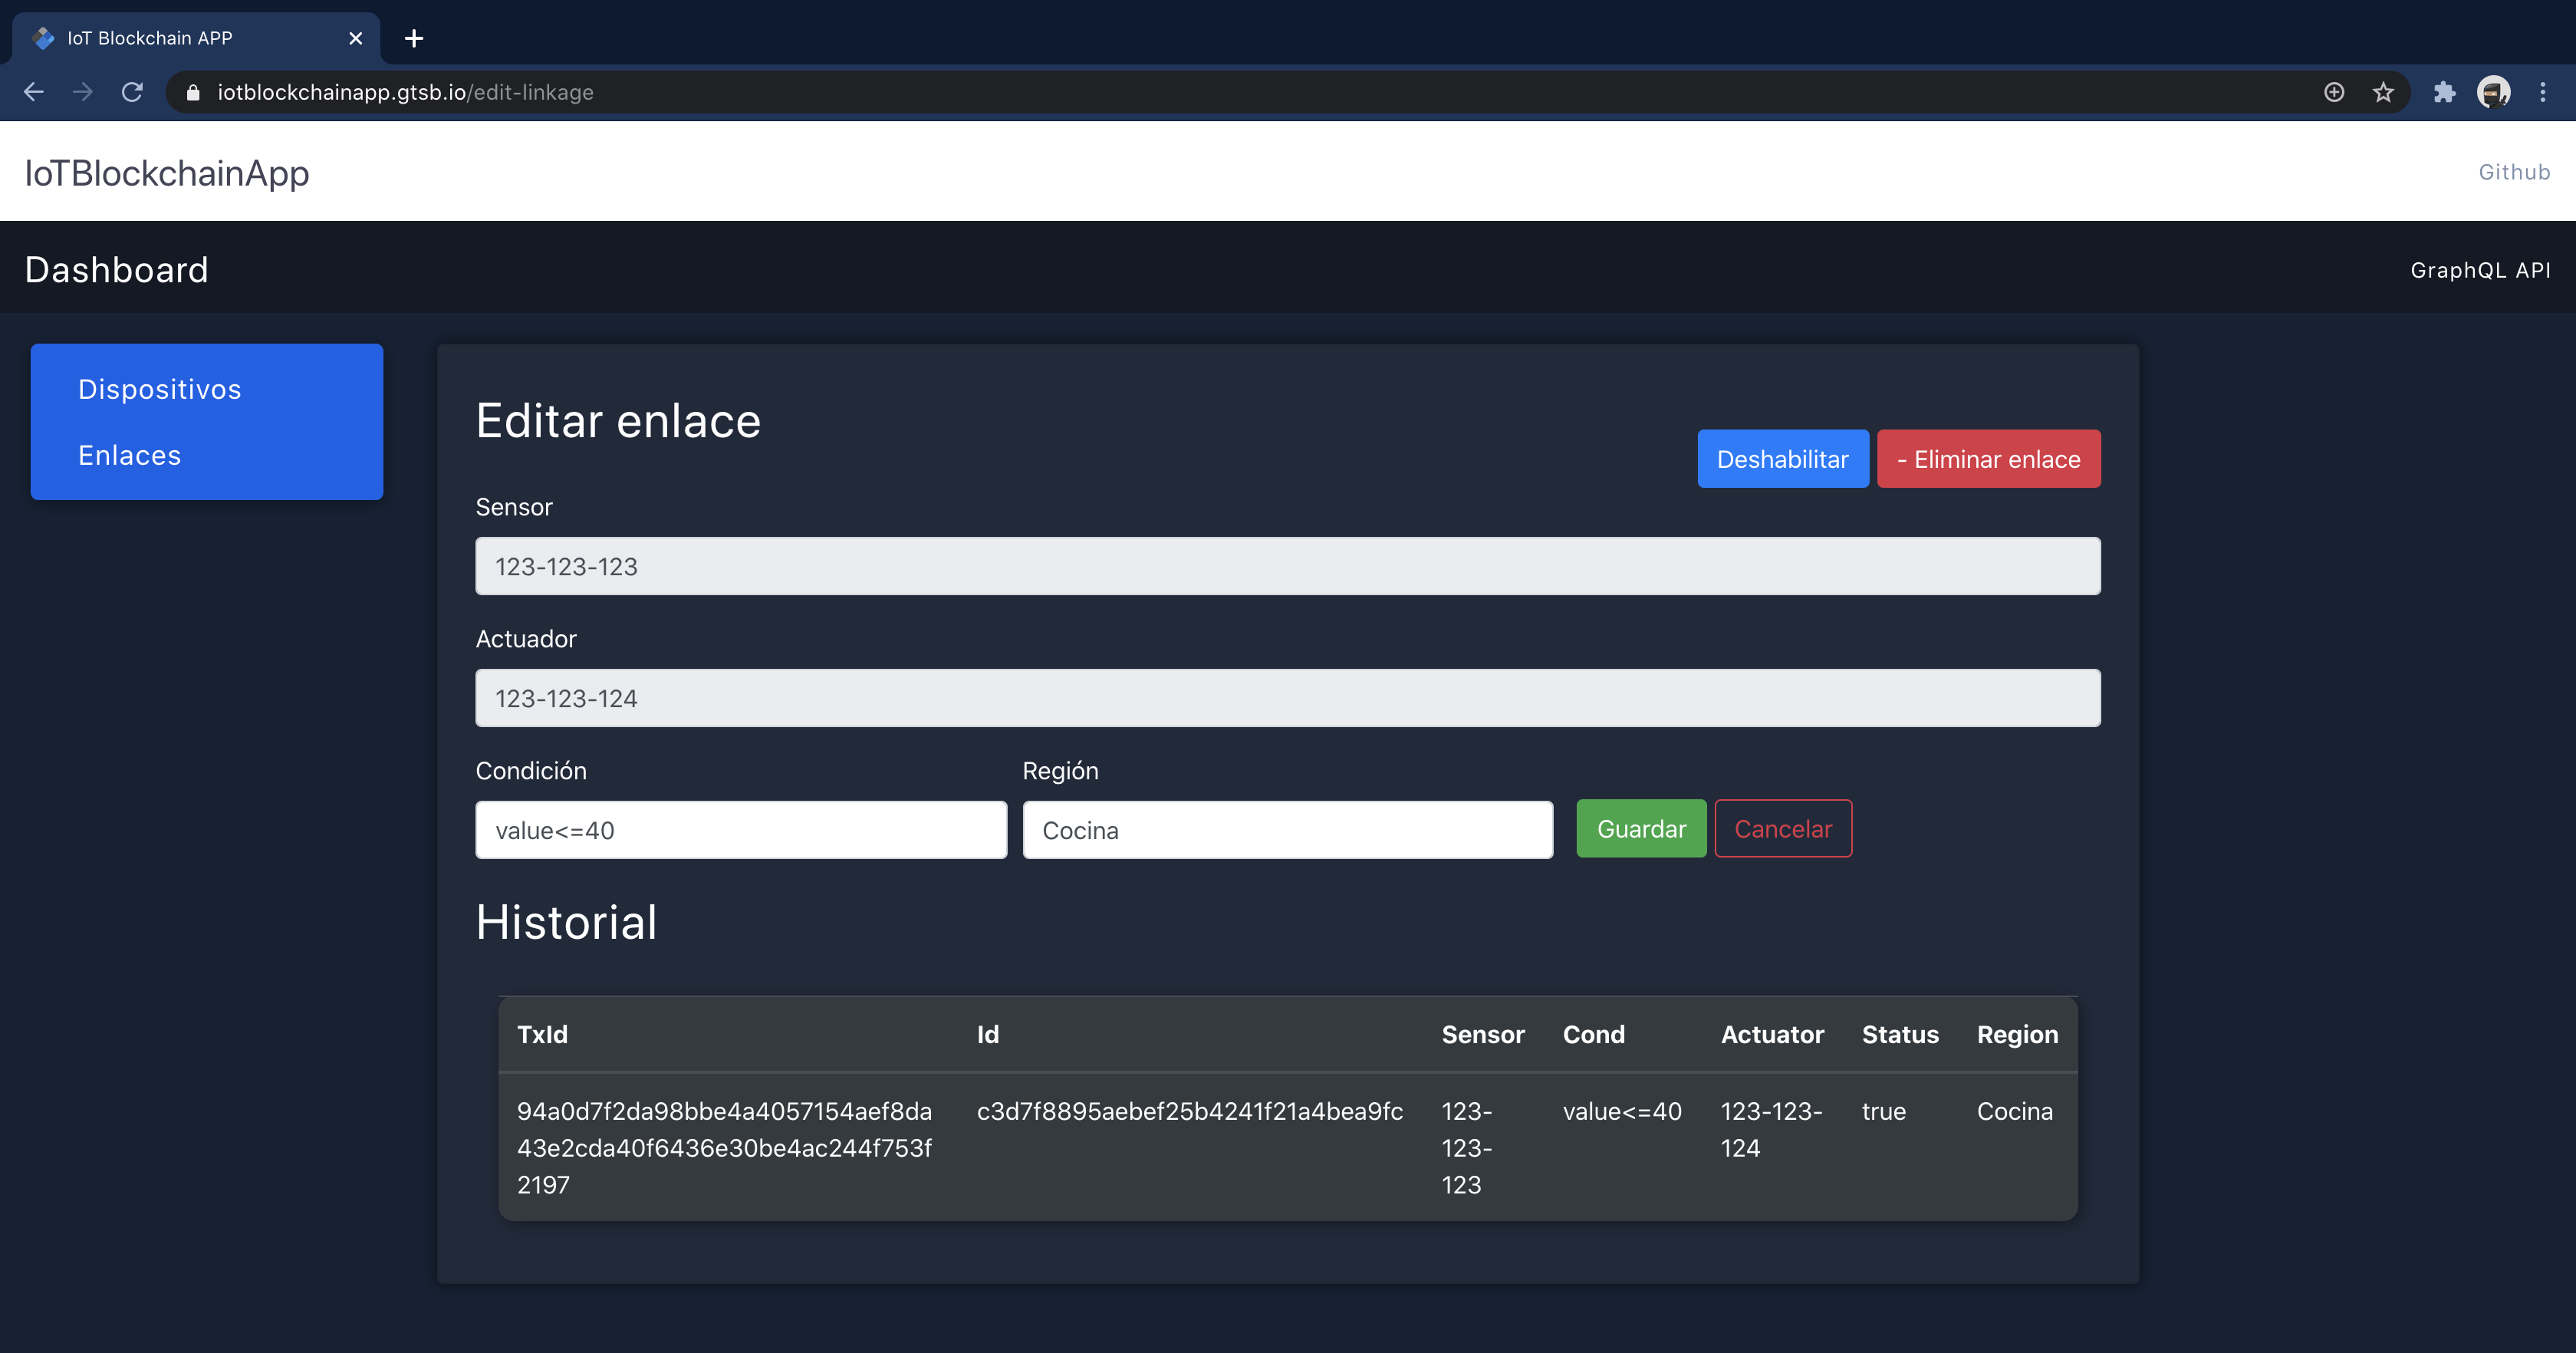
\includegraphics[width=\textwidth]{imagenes/desarrollo/web/editar_enlace}
  \caption{Editar enlace.}
  \label{fig:editar-enlace}
\end{figure}

\subsection{Instalación de PWA.}

\subsubsection*{Portatil.}

\begin{figure}[h!]
 \centering
 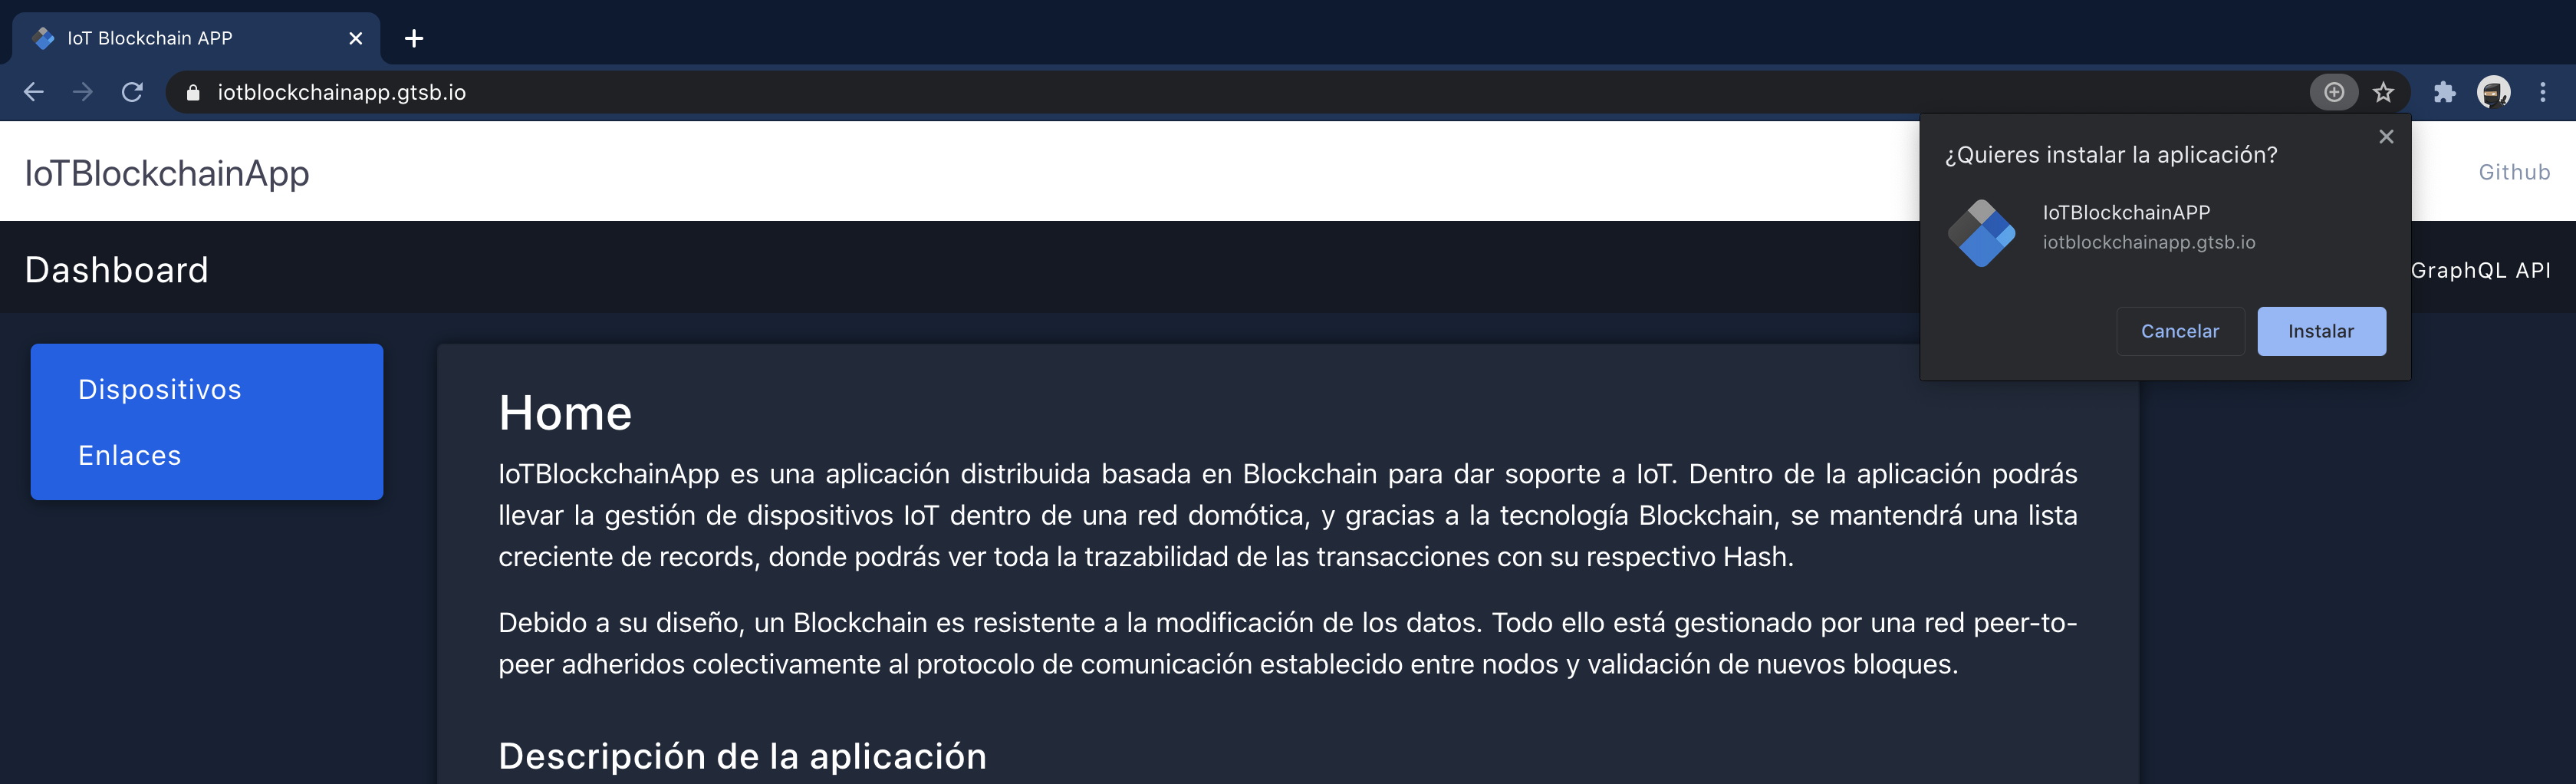
\includegraphics[width=\textwidth]{imagenes/desarrollo/web/pwa/instalacion_pwa_portatil}
 \caption{Instalación PWA en portatil.}
 \label{fig:instalacion-pwa-portatil}
\end{figure}

\begin{figure}[t!]
  \centering
  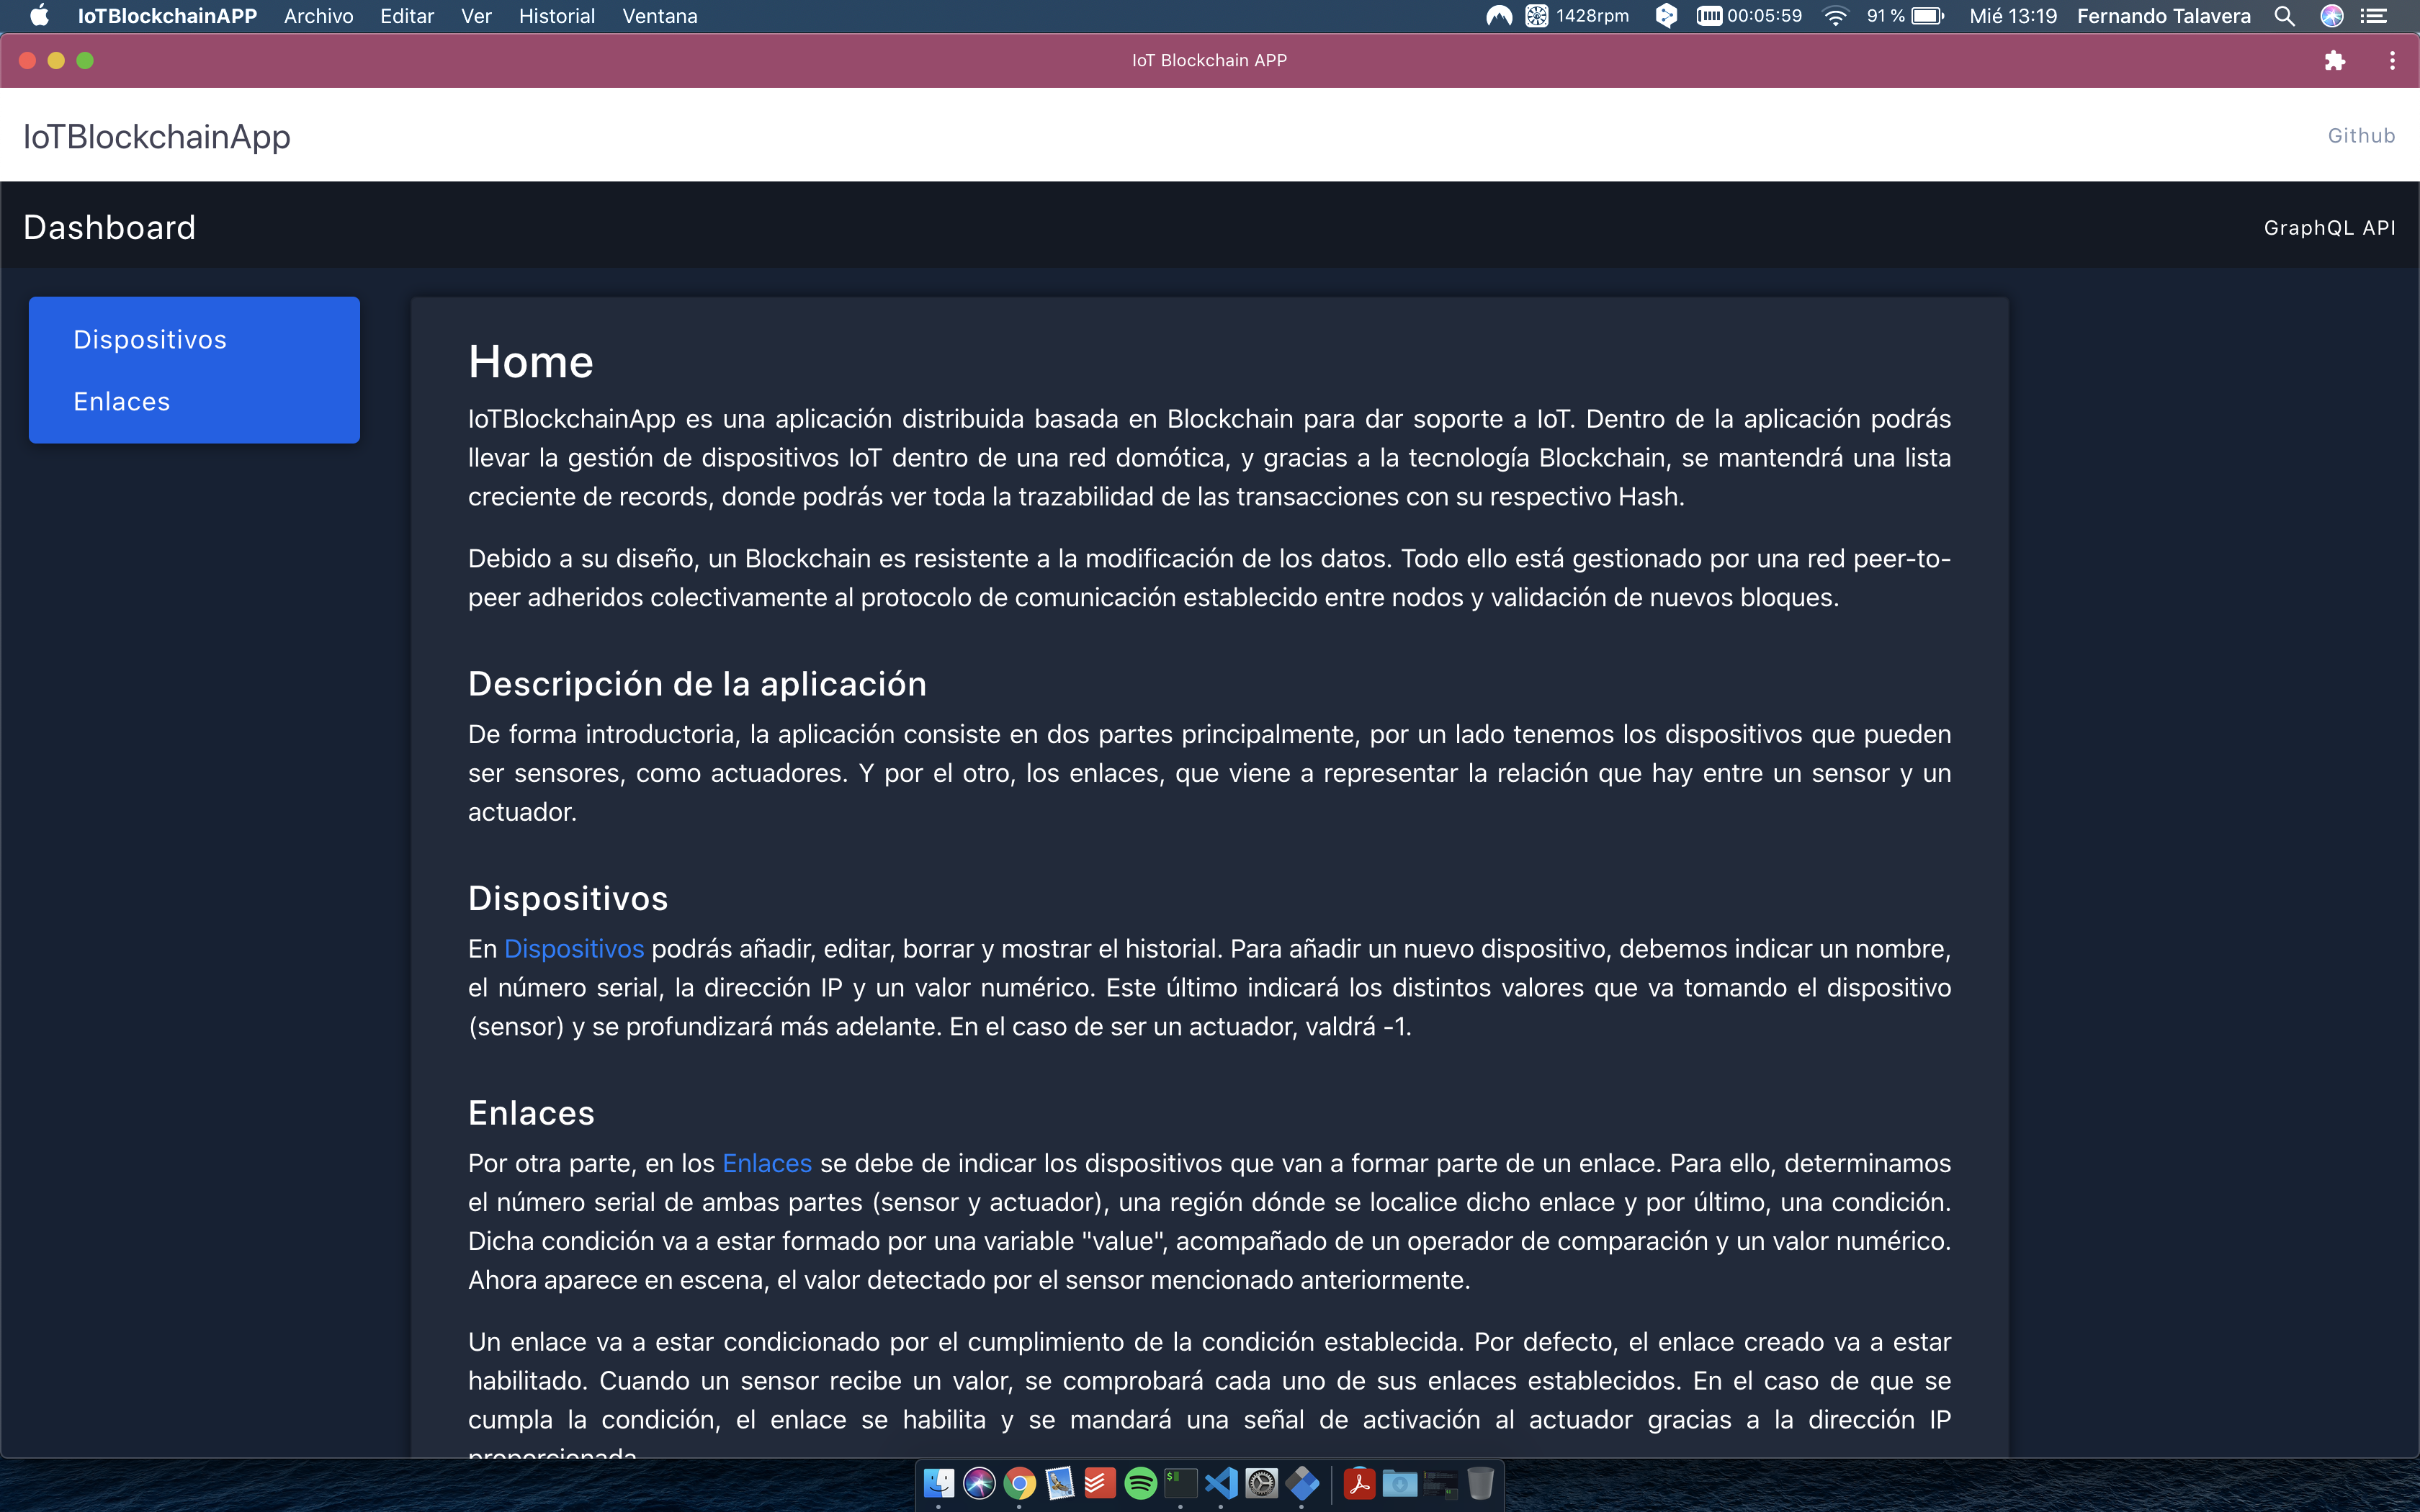
\includegraphics[width=\textwidth]{imagenes/desarrollo/web/pwa/app_portatil}
  \caption{App PWA en portatil.}
  \label{fig:app-portatil}
\end{figure}

\subsubsection*{Móvil.}

\begin{figure}[h!]
  \begin{subfigure}{0.5\textwidth}
    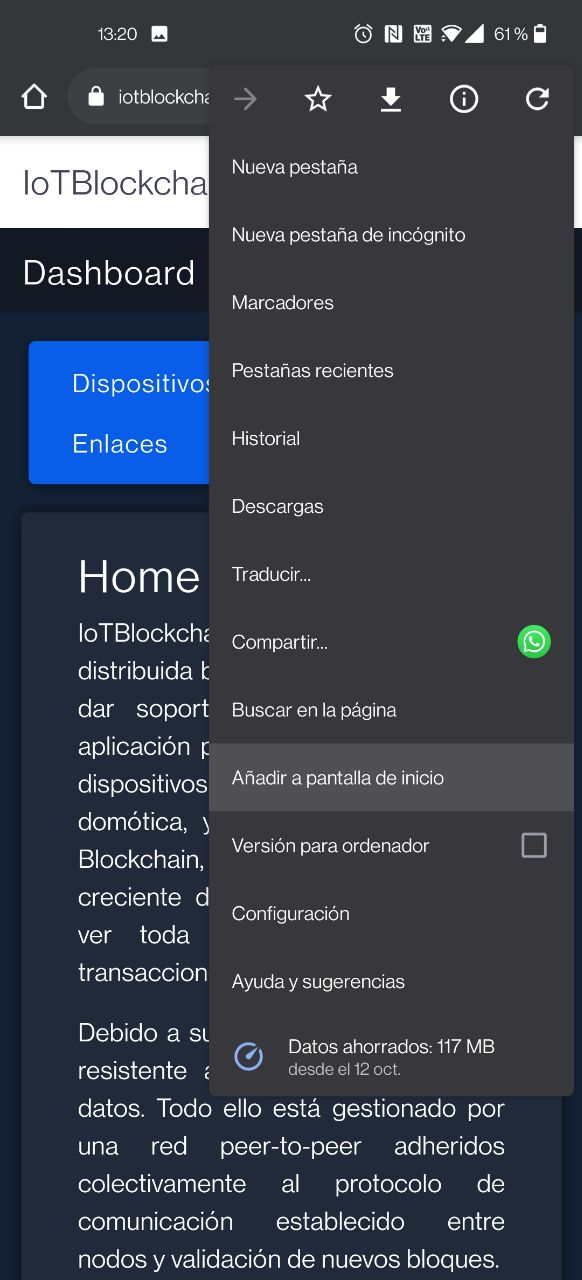
\includegraphics[width=\linewidth]{imagenes/desarrollo/web/pwa/instalacion_pwa_movil1}
    \caption{Instalación PWA en móvil parte 1.}
    \label{fig:instalacion-pwa-movil1}
  \end{subfigure}
  \begin{subfigure}{0.5\textwidth}
    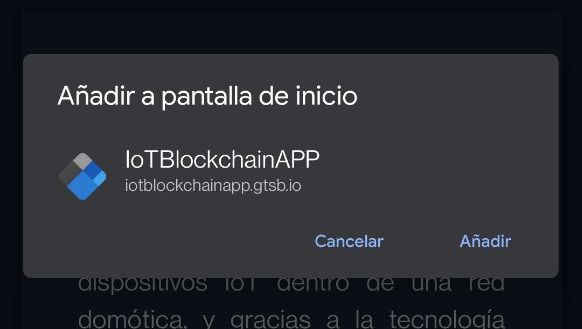
\includegraphics[width=\linewidth]{imagenes/desarrollo/web/pwa/instalacion_pwa_movil2}
    \caption{Instalación PWA en móvil parte 2.}
    \label{fig:instalacion-pwa-movil2}
  \end{subfigure}
  \caption{Instalación PWA en móvil.}
  \label{fig:instalacion-pwa-movil}
\end{figure}

\begin{figure}[h!]
  \begin{subfigure}{0.5\textwidth}
    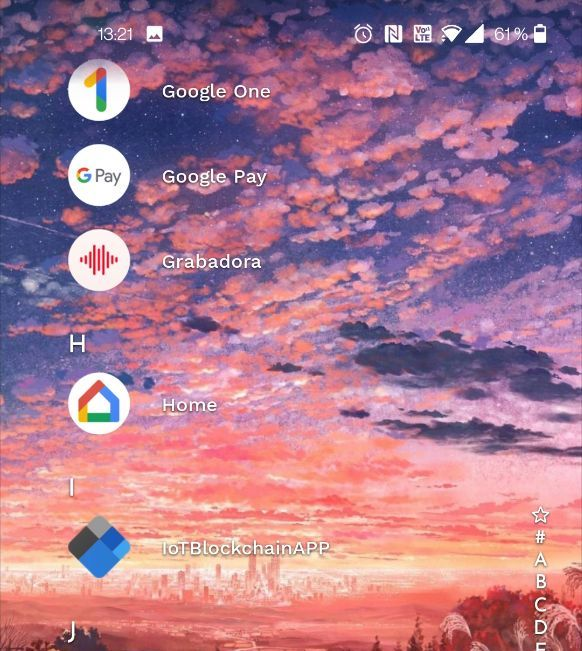
\includegraphics[width=\linewidth]{imagenes/desarrollo/web/pwa/icon_app}
    \caption{Icono de la aplicación en el móvil.}
    \label{fig:icon-app}
  \end{subfigure}
  \begin{subfigure}{0.5\textwidth}
    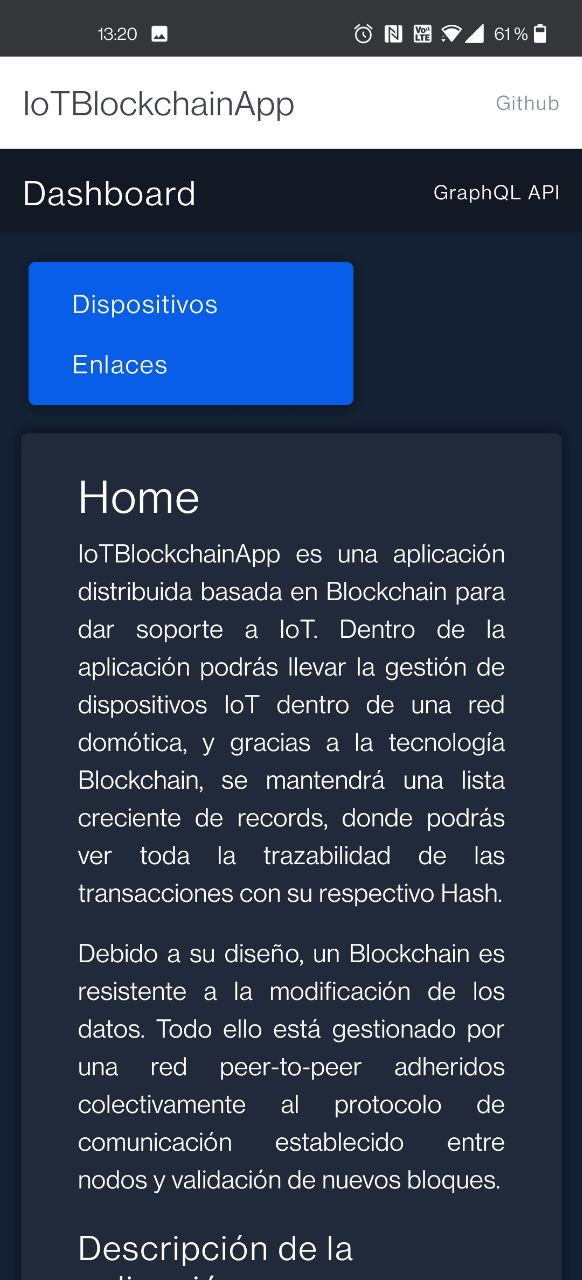
\includegraphics[width=\linewidth]{imagenes/desarrollo/web/pwa/app_movil}
    \caption{App PWA en movil.}
    \label{fig:app-movil}
  \end{subfigure}
  \caption{Aplicación móvil.}
  \label{fig:aplicacion-movil}
\end{figure}

\newpage